
\documentclass[../main.tex]{subfiles}
\begin{document}

\chapter{Background}
\label{ch:background}

\section{Mathematical background}
\label{sec:tda}
This section provides the necessary mathematical background to comprehend the methods proposed in \cite{hofer_densified_2021, moschella_relative_2022} and the ones described in Chapter~\ref{ch:methods}. The exposition is mainly based on \cite{edelsbrunner_computational_2010}.

\subsection{Simplicial Complexes}
\subsubsection*{Geometric simplicial complexes}

As discussed in the introduction, our objective is to analyze the characteristics of the underlying manifold from which our dataset has been sampled. To achieve this, we aim to introduce structure to our dataset that allows us to assess the desired topological properties.

One approach to represent topological spaces is through decomposition into simpler pieces. A decomposition is referred to as a complex if its pieces are topologically simpler and their intersections are of the same type, but lower dimensional \cite{edelsbrunner_computational_2010}. There exists a wide variety of complexes with different levels of abstraction. However, our focus will be on simplicial complexes, which can represent most spaces encountered in data science and are particularly advantageous from a computational standpoint.\\

Simplicial complexes can be studied from both geometric and combinatorial perspectives. In this subsection, we will examine their definition and main properties from a geometric viewpoint. To this end, it will be helpful to review the following concepts from affine geometry.

\begin{definition}
A subset of points $\{u_0, u_1, ..., u_k\} \subseteq \RR^d$ is \emph{affinely independent} if the vectors $\{\overrightarrow{u_0u_1}, ..., \overrightarrow{u_0u_k}\}$ are linearly independent.
\end{definition}

\begin{definition}
\begin{sloppypar}
Given ${u_0, u_1, ..., u_k} \subseteq \RR^d$, we say that $x \in \RR^d$ is a \emph{convex combination} of these points if $x = \sum_{i=0}^{k} \lambda_i u_i$, where $\lambda_i \geq 0$ for all $i \in {0,...,k}$ and $\sum_{i=0}^{k} \lambda_i = 1$.
\end{sloppypar}
\end{definition}

\begin{definition}
\begin{sloppypar}
The \emph{convex hull} of $u_0, u_1, ..., u_k$, denoted by ${\text{conv}{u_0, u_1, ..., u_k}}$, is the set of all convex combinations of the given points.
\end{sloppypar}
\end{definition}

Using these concepts, we can define the building blocks of our decomposition as follows:

\begin{definition}
A \emph{$k$-simplex} $\sigma$ in $\RR^d$ with $d \geq k$ is the convex hull of $k+1$ affinely independent points $u_0, u_1, ..., u_k \in \RR^d$, i.e.,
$\sigma \coloneqq \text{conv}\{u_0, u_1, ..., u_k\}$.
\end{definition}

We say that the $k$-simplex $\sigma$ has dimension $k$, and the points $u_0, u_1, ..., u_k$ are referred to as the \emph{vertices of $\sigma$}.

\begin{figure}[h]
\centering
\begin{subfigure}[b]{0.2\textwidth}
\centering
   
\begin{tikzpicture}[thick, scale=0.7]
    	\tikzstyle{point}=[circle,thick,draw=black,fill=black,inner sep=0pt,minimum width=4pt,minimum height=4pt]
    	\node (a)[point] at (0,0) {};
    \end{tikzpicture}
    \caption{0-simplex}\label{fig:0simp}
\end{subfigure}
\begin{subfigure}[b]{0.2\textwidth}
\centering
	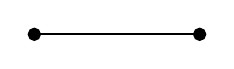
\begin{tikzpicture}[thick, scale=0.7]
    	\tikzstyle{point}=[circle,thick,draw=black,fill=black,inner sep=0pt,minimum width=4pt,minimum height=4pt]
    	\node (a)[point] at (0,0) {};
    	\node (b)[point] at (3,0) {};
 
    	\draw (a.center) -- (b.center) --cycle;
	\end{tikzpicture}
	\caption{1-simplex}\label{fig:1simp}
\end{subfigure}\hspace{0.05\textwidth}
\begin{subfigure}[b]{0.2\textwidth}
\centering
	\begin{tikzpicture}[thick, scale=3]
    	\tikzstyle{point}=[circle,thick,draw=black,fill=black,inner sep=0pt,minimum width=4pt,minimum height=4pt]
    	\coordinate (a) at (0,0);
    	\coordinate (b) at (1,0);
    	\coordinate (c) at (0.6,0.5);

    	\draw[fill=greeo,opacity=0.6] (a) -- (b) -- (c) -- cycle;
 
    	\draw (a) -- (b) -- (c)  --cycle;
    	
    	\node ()[point] at (a) {};
    	\node ()[point] at (b) {};
    	\node ()[point] at (c) {};
	\end{tikzpicture}
	\caption{2-simplex}\label{fig:2simp}
\end{subfigure}\hspace{0.05\textwidth}
\begin{subfigure}[b]{0.2\textwidth}
\centering
	\begin{tikzpicture}[thick,scale=3]
    	\tikzstyle{point}=[circle,thick,draw=black,fill=black,inner sep=0pt,minimum width=4pt,minimum height=4pt]

	\coordinate (A1) at (0,0);
	\coordinate (A3) at (1,0);
	\coordinate (A4) at (0.4,-0.3);
	\coordinate (B1) at (0.5,0.5);

	\draw[thick,dashed,opacity=0.6] (A1) -- (A3);
	\draw[fill=greeo,opacity=0.6] (A1) -- (A4) -- (B1) -- cycle;
	\draw[fill=greeo,opacity=0.6] (A3) -- (A4) -- (B1) -- cycle;

	\draw (A1) -- (B1)  -- (A3) -- (A4) --(A1) --cycle;
	
	\node ()[point] at (A1) {};
	\node ()[point] at (A3) {};
	\node ()[point] at (A4) {};
	\node ()[point] at (B1) {};
	\end{tikzpicture}
	\caption{3-simplex}\label{fig:3simp}
\end{subfigure}
\caption{Representation of 0, 1, 2, and 3-dimensional simplices}
\end{figure}

We can see that any subset of the vertices of $\sigma$ will be affinely independent and will therefore define a lower dimensional simplex $\tau$. Hence, we will say that \emph{$\tau$ is a face of $\sigma$} if it is a convex combination of a non-empty subset of the vertices of $\sigma$, and we will denote it by $\tau \leq \sigma$. If the subset is proper, we will say that \emph{$\tau$ is the proper face of $\sigma$}, and we will denote it by $\tau < \sigma$.\\

Based on the concept of faces, we can establish the notions of the \emph{boundary and interior} of a simplex $\sigma$.

\begin{definition}
Let a simplex $\sigma$. Then we define
\begin{itemize}
	\item \emph{boundary of $\sigma$} as \[\text{bd } \sigma = \bigcup_{\tau<\sigma}\tau\,.\]
	\item \emph{interior of $\sigma$} as \[\text{int }\sigma= \sigma - \text{bd }\sigma\,.\]
\end{itemize}
\end{definition}

Now that we have established the components of our decomposition, we need to understand how to combine them and explore the main properties of the resulting complexes.

As previously mentioned, for a decomposition to be considered a complex, its components must be topologically simple, and the intersections between them should yield lower-dimensional components of the same type. The most natural way to achieve this is by gluing simplices together using their faces.

\begin{definition}
A \emph{simplicial complex} is a finite collection of simplices $K$ that satisfy the following properties:
\begin{enumerate}
	\item If $\sigma \in K$ and $\tau \leq \sigma$ then $\tau \in K$.
	\item If $\sigma_0,\sigma_1 \in K$ and $\sigma_0 \cap \sigma_1 \neq \emptyset$ then $\sigma_0 \cap \sigma_1 \leq \sigma_i$ for $i = 1,2$.
\end{enumerate}
\end{definition}

We define the dimension of $K$ as the maximum of its simplices dimensions.

We can see in Figure~\ref{fig:comp1} an example of a simplicial complex, while Figure~\ref{fig:noComp} shows an example of something that does not verify the abovementioned properties.

\begin{figure}[ht]
\centering
\begin{tikzpicture}[thick,scale=3]
    	\tikzstyle{point}=[circle,thick,draw=black,fill=black,inner sep=0pt,minimum width=4pt,minimum height=4pt]

	\coordinate (x) at (0,0);

	\coordinate (A1) at (1,0);
	\coordinate (A3) at (2, 0.1);
	\coordinate (A4) at (1.4,-0.3);
	\coordinate (B1) at (1.5,0.5);

    \coordinate (b) at (3,0);
    \coordinate (c) at (2.6,-0.5);
    
    \coordinate (a1) at (3.4,0.12);
    \coordinate (b1) at (4,0);
    \coordinate (c1) at (3.8,0.3);
    
    \coordinate (y) at (3.5,-0.4);
	
	\draw[thick,dashed,opacity=0.6] (A1) -- (A3);
    \draw[fill=greeo,opacity=0.6] (a1) -- (b1) -- (c1) -- cycle;
	\draw[fill=greeo,opacity=0.6] (A1) -- (A4) -- (B1) -- cycle;
	\draw[fill=greeo,opacity=0.6] (A3) -- (A4) -- (B1) -- cycle;

	\draw (a1) -- (b1) -- (c1)  --cycle;	
	\draw (A1) -- (B1)  -- (A3) -- (A4) --(A1) --cycle;
	\draw (x) -- (A1) --cycle;	
	\draw (A3) -- (b) -- (c)  --cycle;	
	\draw (b1) -- (y) --cycle;
	\draw (B1) -- (A4) --cycle;
	
	\node ()[point] at (x) {};
	\node ()[point] at (A1) {};
	\node ()[point] at (A3) {};
	\node ()[point] at (A4) {};
	\node ()[point] at (B1) {};
    \node ()[point] at (b) {};
    \node ()[point] at (c) {};
    \node ()[point] at (a1) {};
    \node ()[point] at (b1) {};
    \node ()[point] at (c1) {};
    \node ()[point] at (y) {};	
	
	\end{tikzpicture}
\caption{Example of a simplicial complex}
\label{fig:comp1}
\end{figure}

\begin{figure}[ht]
\centering
\begin{tikzpicture}[thick]
    \tikzstyle{point}=[circle,thick,draw=black,fill=black,inner sep=0pt,minimum width=4pt,minimum height=4pt]
    \coordinate (a) at (0,0);
    \coordinate (b) at (3,0);
    \coordinate (c) at (2,2);

    \begin{scope}[yshift=2cm]
    	\coordinate (d) at (1,1);
    	\coordinate (e) at (0,2);
    	\coordinate (f) at (4,2);
    \end{scope}

	\coordinate (p) at (1.5,0.5);

    \draw[fill=greeo,opacity=0.6] (a) -- (b) -- (c) -- cycle;
    \draw[fill=greeo,opacity=0.6] (d) -- (e) -- (f) -- cycle;
    
 
    \draw (p) -- (d) --cycle;
    \draw (a) -- (b) -- (c)  --cycle;
    \draw (d) -- (e) -- (f) -- cycle;    
    
	\node ()[point] at (a) {};
    \node ()[point] at (b) {};
    \node ()[point] at (c) {};
    \node ()[point] at (d) {};
    \node ()[point] at (e) {};
    \node ()[point] at (f) {};
    \node ()[point] at (p) {};    
\end{tikzpicture}
\caption{Example of simplices that does not verify the simplicial complex conditions}
\label{fig:noComp}
\end{figure}

\begin{definition}
The \emph{underlying space} of a simplicial complex $K$, denoted $\abs{K}$, is the union of the simplices in $K$ with the induced topology of $\RR^d$, where the simplex are contained. This underlying space is also called \emph{polyhedron}.
\end{definition}
As can be seen, the underlying space of a simplicial complex is compact since it is a finite union of simplices. The following result characterizes the open and closed sets of the underlying space $\abs{K}$ of a simplicial complex $K$.

\begin{proposition}[{\cite[Chapter~3]{edelsbrunner_computational_2010}}]
Let $K$ be a simplicial complex and $A \subset \abs{K}$ a subset. Then $A$ is an open (closed) set in $K$ if and only if for every $\sigma \in K$, $A \cap \abs{\sigma}$ is an open (closed) set of $\abs{\sigma}$.
\end{proposition}

\begin{definition}
A \emph{triangulation} of a topological space $X$ is a pair $(K, h)$ where $K$ is a simplicial complex and $h: X \to \abs{K}$ is a homeomorphism (i.e., $h $ continuous, bijective and $h^{-1}$ continuous).
\end{definition}
We say that a topological space is \emph{triangulable} if it admits triangulation.\\

It will also be helpful for us to be able to study the simplicial complexes contained in another simplicial complex.
\begin{definition}
A \emph{subcomplex} $L$ of a simplicial complex $K$ is a simplicial complex $L \subseteq K$.
\end{definition}

A particular type of subcomplex that is of great interest is the \emph{$j$-skeletons}, defined as follows: \[K^{(j)} = \{\sigma \in K \mid dim\ \sigma\ \leq j \}\,.\]

\subsubsection*{Abstract simplicial complexes}
Now that we have established the concept of simplicial complexes from a geometric perspective, we will approach them from a combinatorial standpoint, which will significantly aid in the representation and manipulation of simplicial complexes.

\begin{definition}
An \emph{abstract simplicial complex $A$} is a finite collection of finite sets such that if $\alpha \in A$ and $\beta \subset \alpha$, then $\beta \in A$.
\end{definition}
In this way, it is fulfilled that
\begin{itemize}
    \item Non-empty sets in $A$ are called \emph{abstract simplices}.
    \item The \emph{dimension} of an abstract simplex $\alpha \in A$ is $\text{dim}\ \alpha = \text{card}(\alpha) - 1$. And the dimension of the complex is the maximum of the dimensions of its simplices.
    \item A \emph{face} of $\alpha \in A$ is any non-empty subset of $\beta \subset \alpha$.
    \item The \emph{set of vertices} of $A$, denoted by $\text{Vert } A$, is the union of all its simplices.
    \item A \emph{subcomplex $B$} of an abstract simplicial complex $A$ is an abstract simplicial complex $B \subset A$.
\end{itemize}

\begin{exmp}
The following set forms an abstract simplicial complex:

\begin{gather*}
A = \{\{0\},\{1\},\{2\},\{3\},\{4\},\{5\},\{6\},\{0,1\},\{1,2\},\{1,3\},\{1,4\},\{2,3\},\\
\{2,4\},\{3,4\},\{4,5\},\{4,6\},\{5,6\},\\
\{1,2,3\},\{1,2,4\},\{1,3,4\},\{2,3,4\},\{1,2,3,4\}\}\,.
\end{gather*}

Where the set of vertices is: $\text{Vert }A = \{0, 1, 2, 3, 4, 5, 6\}$.
\end{exmp}

\begin{definition}
Let $A$ and $B$ be two abstract simplicial complexes. We say that $A$ and $B$ are \emph{isomorphic} if there exists a bijection $b:\text{Vert }A \to \text{Vert }B$ such that $\alpha \in A$ if and only if $b(\alpha) \in B$.
\end{definition}

Each geometric complex naturally induces an abstract complex as follows:
\begin{definition}
Let $K$ be a simplicial complex, and let $V$ be the set of vertices of $K$. Then, we will call \emph{vertex scheme} the abstract simplicial complex $A$ formed by all those subsets of $V$ that generate simplices in $K$.
\end{definition}

Under certain circumstances, it is possible to construct a (geometric) simplicial complex from an abstract complex:
\begin{definition}
Let $A$ be an abstract simplicial complex and $K$ a simplicial complex. We will say that $K$ is a \emph{geometric realization} of $A$ if $A$ is isomorphic to the vertex scheme of $K$.
\end{definition}

\begin{theorem}[{\cite[Chapter~3]{edelsbrunner_computational_2010}}]
Every abstract simplicial complex of dimension $d$ admits a geometric realization in $\RR^{2d + 1}$.
\end{theorem}

Thus, abstract simplicial complexes provide a faithful representation of (geometric) simplicial complexes.

\subsection{Simplicial complexes built from point clouds}
From the computational point of view, we find ourselves with the problem that we have a representation of a topological space through a finite discretization, and our objective is to be able to recover properties of the original topological space from this cloud of points. Hence, to give some structure to our distance space $(X,d)$, where $X$ is the dataset and $d: X \to \overline{\RR}_+$ is a distance function, we will create a simplicial complex with the data points as vertices, and encoding some of the relevant information of $d$.

\subsubsection*{\v{C}ech complex}
The \v{C}ech complex is defined from the intersection of a collection of disks (closed balls). The idea underlying this construction is that of the nerve of a collection, which is introduced below.

\begin{definition}
Let $F$ be a finite collection of sets. The \emph{nerve} of $F$ is defined as the abstract simplicial complex
\[
{\rm Nrv}\ F= \left\{ X \subseteq F \mid \bigcap_{x\in X} x \neq \emptyset \right\}\,.
\]
\end{definition}

One of the reasons we are interested in simplicial complexes constructed through the nerve of a collection is based on the implications of the following theorem.

\begin{theorem}[Nerve theorem {\cite[Chapter~3]{edelsbrunner_computational_2010}}]
If $F$ is a finite collection of closed and convex subsets in Euclidean space, then the nerve of $F$ has the same type of homotopy as the union of the sets of $F$.
\end{theorem}
Therefore, according to this theorem, \v{C}ech complexes exhibit similar topological properties to subsets of $\mathbb{R}^d$ (as they are homotopy equivalent). This property ensures that our analysis of topological properties obtained through homology groups of the simplicial complex will be equivalent to studying them on neighborhoods of our dataset $X \subset \mathbb{R}^d$ \cite{doherty_cech_2018}.\\

Considering the case where the sets in the collection are disks (closed balls), denoted as $D_r(x) \equiv \overline{B_r}(x) = {y\in \mathbb{R}^d \mid d(x, y) \leq r}$ in $\mathbb{R}^d$, we define the \v{C}ech complex of a finite set of points $X \subset \mathbb{R}^d$ as follows:

\begin{definition}
Let $X\subset \RR^d$ be a finite set of points. We will call \emph{\v{C}ech complex} of $X$ of radius $r$ to the abstract simplicial complex
\[
\text{\v{C}ech}(r)=\left\{\sigma \subset X \mid \bigcap_{u \in \sigma} D_{r/2}(u)\neq \emptyset \right\}\,.
\]
\end{definition}

\begin{figure}[!ht]
\centering
\includegraphics[width=0.5\textwidth]{figures/bg/Cech.png} 
\caption{\v{C}ech complex for a set of nine points and a radius $r$. Source: \cite{edelsbrunner_computational_2010}}
\label{fig:cech}
\end{figure}

We can check that for large enough values of $r$, $\text{\v{C}ech}(r)$ is a simplex of dimension $\text{card }(X)-1$ {\cite[Chapter~3]{edelsbrunner_computational_2010}}, so the \v{C}ech complex is computationally inefficient.

Furthermore, in general, the \v{C}ech complex of a set of points $X \subset \RR^d$ does not possess a geometric realization in $\RR^d$. Therefore, we will present a construction that resembles the \v{C}ech complex while being more computationally favorable.

\subsubsection*{Vietoris-Rips complex}

\begin{definition}
Let $X \subset \RR^d$ be a finite set of points. We call \emph{Vietoris-Rips} complex of $X$ of radius $r$ to the abstract simplicial complex 
\begin{align*}
\text{VR}(X, r) =& \{\sigma \subseteq  X \mid \textrm{diam } \sigma \leq r\}\\
=&\left\{ \{x_0, ..., x_n\} \subseteq  X \mid d(x_i, x_j) \leq r\ \forall i,j\right\}\,. 
\end{align*}
If the set $X$ is understood from the context, then we can note it as $\text{VR}(r)$.
\end{definition}

We can see in Figure~\ref{fig:vr} how the various VR complexes are generated as the radius increases.

\begin{figure}[!ht]
\centering
\includegraphics[width=0.9\textwidth]{figures/bg/vr.png} 
\caption{Vietoris-Rips complexes for a set of seven points as we increase the radius from left to right. Source: \cite{ulmer_topological_2019}}
\label{fig:vr}
\end{figure}

Let $\sigma \subset X$, then we recall that the diameter is defined as
\[\textrm{diam } \sigma = \max_{u,v \in \sigma} d(u,v)\,.\]
It follows that $\sigma \in \text{VR}(r)$ if and only if all its edges are in $\text{VR}(r)$. In other words, the Vietoris-Rips complex is entirely determined by its $1$-skeleton. This property makes the Vietoris-Rips complex computationally more efficient than the \v{C}ech complex. However, similar to the \v{C}ech complex, the Vietoris-Rips complex does not admit a geometric realization in $\RR^d$.

On the other hand, the Vietoris-Rips complex is not the nerve of any collection of subsets of $\RR^d$. Nevertheless, the following result guarantees that the VR complex provides an approximation of the \v{C}ech complex:

\begin{lemma}[Vietoris-Rips lemma {\cite[Chapter~3]{edelsbrunner_computational_2010}}]
\label{fig:lemaVR}
Let $X \subset \RR^d$ be a finite set of points and let $r \geq 0$. Then,
\[
\text{\rm \v{C}ech}(r) \subset \text{\rm VR}(r) \subset \text{\rm \v{C}ech}(\sqrt{2}r)\,.
\]
\end{lemma}

Another important property regarding VR complexes is their ability to encode $\epsilon$-connectivity. In Section~\ref{sec:topoML}, we will talk more in detail about $\epsilon$-connectivity and how it will be a crucial property for constructing our topological regularization. 

\begin{definition}[\cite{robins_resolutions_2000}]
We say that a metric space $X$ is \emph{$\epsilon$-disconnected} if there exist two subsets $U$ and $V$ with $U\cup V = X$, and $d(U,V)\equiv \inf_{x\in U,\, y\in V}d(x,y) > \epsilon$.
\end{definition}
Hence if the space is not $\epsilon$-disconnected, we will say that $X$ is $\epsilon$-connected. Moreover, a subset $A \subset X$ is an \emph{$\epsilon$-component} if $A$ is $\epsilon$-connected and $d(A, {X \setminus A}) > \epsilon$. Hence, for any given $\epsilon$, we can decompose our dataset $X$ in disjoint $\epsilon$-components.

However, to see the connection of VR complex with $\epsilon$-connectivity, we will use another definition based on \emph{$\epsilon$-chains}.

\begin{definition}[\cite{robins_resolutions_2000}]
We call \emph{$\epsilon$-chain} to a finite sequence of points $x_0, .., x_n$ such as $d(x_i, x_{i+1})\leq \epsilon$ for $i=1,...,n$. 
\end{definition}

Therefore, for any set $X$, if we can form an \emph{$\epsilon$-chain} between any pair of points, then our set is $\epsilon$-connected. 

\begin{proposition}
\label{prop:connected}
For any distance $d$ on $X$, and $\epsilon \geq 0$, the partition corresponding to the connected components of $\text{\rm VR}(\epsilon)$, denoted as $\pi_0(\text{\rm VR}(\epsilon))$, coincides with the $\epsilon$-components of $X$.
\end{proposition}

This result follows easily from the fact that two points $u,v$ (vertices) are in the same connected component of a simplicial complex $K$ if there exists a sequence of vertices $u=x_0,..., x_n=v$ such as $\{x_i, x_{i+1}\} \in K$. So, we can see that in the case that $K$ is a Vietoris-Rips complex of radius $\epsilon$, then $\{x_i, x_{i+1}\} \in K$ iff $d(x_i, x_{i+1})\leq\epsilon$, i.e, there exist an $\epsilon$-chain between $u$ and $v$. 

\subsubsection*{Witness complex}

A common ML scenario is that we will have a big dataset, and we apply our training procedure to small batches of that given set. Hence, ideally, we would want to be able to infer the topology of our whole dataset just from studying our reduced batches. Therefore, this type of ideas motivated Vin de Silva and Gunnar Carlsson when they introduced the Witness Complex in \cite{silva_topological_2004}: a subset of the data points, called the landmarks points, is used to construct the simplices ``seen'' by the witnesses, which are the rest of the points of the data set \cite{medbouhi_towards_2022}.

However, the construction of the simplicial complex that we will use differs from the ones used in standard TDA libraries, such as GUDHI, when defining Witness complexes \cite{noauthor_gudhi_nodate}. We will focus on a specific type of complex presented in \cite{silva_topological_2004}, which can be seen as an example of a Dowker complex\footnote{Denoted as $W(D; R, 0)$ in the original paper \cite{silva_topological_2004}, and usually called ``lazy witness complexes''}.

\begin{definition}[\cite{dowker_homology_1952}]
The \emph{Dowker complex} of a relation $(R, X, Y)$ is the simplicial complex $(\text{D}(R)), X)$ where
\[
\text{D}(R) = \{\sigma \subseteq X \mid \exists y \in Y \text{ with } \sigma \times \{y\} \subseteq R\}\,.
\]
We say that \emph{the simplex $\sigma \in \text{D}(R)$ is witnessed by $y \in Y$} if $\sigma \times \{y\} \subseteq R$, i.e., all elements in the simplex $\sigma$ are related with y.
\end{definition}

We will call Lazy Witness complex the Dowker complex of $(R_\epsilon, L, X)$ where
\begin{itemize}
    \item $X$ is the whole dataset,
    \item $L\subseteq X$ is a batch, and
    \item $R_\epsilon=\{(l,x)\in L \times X \mid d(l,x)<\epsilon\}$. 
\end{itemize}

\begin{definition}[Nested family of witness complexes \cite{silva_topological_2004}]
\label{def:witness}
Let $(\mathcal{X}, d)$ be a metric space, $X \subset \mathcal{X}$ be a dataset, $L = \{l_0, ..., l_n\} \subseteq X$ be a set of landmark points, and $\epsilon>0$. Then the $k$-simplex $\sigma = \{u_1, ..., u_k\}$ with $u_i \in L$ belongs to the \emph{Lazy Witness complex} $\text{W}_\epsilon(X, L)$ iff all its faces belong to $\text{W}_\epsilon(X, L)$ and there is a witness $x \in X$, such that:
\[
\max \{d(u_i, x) \mid u_i \in \{u_1, ..., u_k\}\} \leq \epsilon\,.
\]
\end{definition}

\begin{figure}[!ht]
\centering
\includegraphics[width=0.9\textwidth]{figures/bg/witnessCons.png} 
    \caption{Witness complex for a set  dataset of 11 points using a subset of 5 landmarks points and radius $\epsilon$. Adapted from: \cite{medbouhi_towards_2022}}
\label{fig:witnessCons}
\end{figure}

A remarkable result about witness complexes is Dowker's Theorem, which states that exchanging the role of the witnesses and landmarks doesn't change the topology of the complex \cite{dowker_homology_1952}. This result is exploited in \cite{schonenberger_witness_2022} to enforce the topological regularization of a Topological Autoencoder (further explained in Section~\ref{sec:topoML}) only using the data points of the batches instead of the whole dataset.

\begin{proposition}[\cite{silva_topological_2004}]
\label{prop:witness-vr}
The family of complexes $\text{\rm W}_\epsilon(X, L)$ is closely related to the family $\text{\rm VR}(L, \epsilon)$. Specifically, there are inclusions:
\[
\text{\rm W}_\epsilon(X, L) \subseteq \text{\rm VR}(L, 2\epsilon) \subseteq \text{\rm W}_{2\epsilon}(X, L)\,.
\]
\end{proposition}

\subsection{Homology}
As can be seen in \cite{hatcher_algebraic_2002}, the homotopy is an algebraic tool to obtain properties of topological spaces. However, the methods for calculating the homotopy are not computationally manageable. Thus, homology is proposed as an algebraic formalism, which, although it is not capable of obtaining as much topological information about space as with other formalisms, is highly beneficial from a computational perspective.

We will start by reviewing some linear algebra concepts that will be useful to understand homology's formal definition fully.

\subsubsection*{Linear algebra interlude}
This subsection is based on Wojciech Chachólski's lecture notes from his course on Topological Data Analysis \cite{chacholski_sf2956_2022}.\\

In TDA we tend to use vector spaces over $F_2$, the field with 2 elements $\{0,1\}$. This field is isomorphic to $\mathbb{Z}_2 \equiv \mathbb{Z}/2\mathbb{Z}$ with operations modulo 2:
\[
0+0 = 0;\ 1+0 = 1;\ 1+1 = 0;\ 1 \cdot 0 = 0;\ 1\cdot 1 = 1\,.
\]

We recall that an $F_2$ vector space is a set $V$ with a zero element $0 \in V$ and an addition operation $V \times V \ni (v,w) \mapsto v+w \in V$ such that, for any $u,v,w$ in $V$:
\begin{itemize}
    \item $v + w = w + v$,
    \item $(v + u) + w = v + (u + w)$,
    \item $0 + v = v$,
    \item $v + v = 0$.
\end{itemize}

Another vector spaces that we will use are \emph{quotient spaces}. Let $W \subset V$ be a vector subspace. We define the following equivalence relation: we say that two elements $v$ and $w$ in $V$ are \emph{equivalent modulo} $W$ if $v-w \in W$. As we can see in Figure~\ref{fig:quot_ex}, the equivalence classes are of the form $[v]=v+W \subset V$. Moreover, the set of equivalence classes, denoted by $V/W$, with the following operations, is a vector space:
\begin{itemize}
    \item $(v+W)+(w+W)=v+w+W$,
    \item $0 = 0 +W = W$,
    \item $a(v+W)=av +W$.
\end{itemize}

\begin{figure}[ht!]
    \centering
    \begin{tikzpicture}[line cap=round,line join=round,>=triangle 45,x=1cm,y=1cm]
        \begin{axis}[
        x=1cm,y=1cm,
        axis lines=middle,
        ymajorgrids=true,
        xmajorgrids=true,
        xmin=-3.5771885955480864,
        xmax=4.11169202904735,
        ymin=-2.6112285059644633,
        ymax=3.610515886376021,]
        \clip(-3.5771885955480864,-2.6112285059644633) rectangle (4.11169202904735,3.610515886376021);
        \draw [line width=2pt,color=qqqqff,domain=-3.5771885955480864:4.11169202904735] plot(\x,{(--8.32--4*\x)/4});
        \draw [line width=2pt,color=wwzzqq,domain=-3.5771885955480864:4.11169202904735] plot(\x,{(--15.76--4*\x)/4});
        \draw [line width=2pt,color=ffqqqq,domain=-3.5771885955480864:4.11169202904735] plot(\x,{(-8.4--4*\x)/4});
        \draw [->,line width=1pt,color=qqqqff] (0,0) -- (-1.04,1.04);
        \draw [->,line width=1pt,color=wwzzqq] (0,0) -- (-0.6041708999218006,3.3358291000781994);
        \draw [->,line width=1pt,color=ffqqqq] (0,0) -- (2.1,0);
        \draw [line width=2pt,domain=-3.5771885955480864:4.11169202904735] plot(\x,{(-0--4*\x)/4});
        \begin{scriptsize}
        \draw[color=black] (-2.2934443923249974,-1.9829409990960194) node {$W$};
        \draw[color=qqqqff] (-2.7,-1.2) node {$[u]$};
        \draw[color=wwzzqq] (-2.7,0.6) node {$[v]$};
        \draw[color=ffqqqq] (0.5,-2.125579243898585) node {$[w]$};
        \draw[color=qqqqff] (-0.6,0.4) node {$u$};
        \draw[color=wwzzqq] (-0.6,2.248660263380096) node {$v$};
        \draw[color=ffqqqq] (1.075535103964169,0.15) node {$w$};
        \end{scriptsize}
        \end{axis}
    \end{tikzpicture}
    \caption{Quotient space example: $\RR^2/W$}
    \label{fig:quot_ex}
\end{figure}

Lastly, we will see that one of our main components for constructing homology is by ``transforming'' a set to a vector space. Hence, for any finite set $X$, and field $F$, we define $FX \equiv \oplus_{x \in X} K$. The vector space $FX$ is isomorphic to $F^{\abs{X}}$, which means that we can represent an element of $FX$ as sequences $(k_x)_{x \in X}$ indexed by elements of X.

\begin{exmp}
Let the set $S=\{a, b, c\}$, and the field $\mathbb{Z}_3$. Then an element of $\mathbb{Z}_3S$ can be
\[
( \underbrace{1}_\text{a}, \underbrace{0}_\text{b}, \underbrace{2}_\text{c}) = 1 \cdot a + 0 \cdot b + 2 \cdot c = a + 2c\,.
\]
\end{exmp}

Therefore, we can see that we can define a basis for this space formed by elements $e_x$, where

\[
(e_x)_y = \left\{\begin{matrix}
1 & \text{ if } y=x\\
0 & \text{ if } y \neq x\\
\end{matrix}\right.
\]

So the notation that we have seen in the example of representing an element as a (unique) linear combination $\sum_{x \in X} a_x x$ can be formalized if we identify each element $x$ in $X$ with $e_x$. Furthermore, given two elements $c = \sum_{x \in X} a_x x$ and $c' = \sum_{x \in X} b_x x$, their sum is defined as
\[
c + c' = \sum_{x \in X} (a_x + b_x) x\,.
\]

Lastly, we will see that we can extend a map of sets $g:X \to Y$ to a linear equation $Fg: KX \to KY$ such as an element $\sum_{x \in X} a_x x$ will be mapped to $\sum_{x \in X} a_x g(x)$.


\subsubsection*{Chain groups}
We will begin by studying the various groups that are involved in the definition of homology.


Let $K$ be a simplicial complex, $F$ a field, and $p$ be a non-negative integer. A \emph{$p$-chain} in $K$ is equal to $FK$. More specifically, $c$ is a $p$-chain in $K$ if
\[
c = \sum a_i\sigma_i
\]
with $\sigma_i$ is a $p$-simplex for each $i$ and $a_i$ are the \emph{coefficients}. These coefficients can be taken from any commutative ring $F$; however, we will use coefficients in the field of two elements, i.e.,  $a_i \in \mathbb{Z}_2$.

\begin{exmp}
We will write the simplices as the list of their vertices, $\sigma = [u_0, u_1, ..., u_p]$.
\begin{itemize}
	\item In the figure~\ref{fig:0cad} the $0$-chain $c=[0]+[2]+[6]+[9]$ is shown in red.
\begin{figure}[!ht]
\centering
\begin{tikzpicture}[thick,scale=3]
    	\tikzstyle{point}=[circle,thick,draw=black,fill=black,inner sep=0pt,minimum width=4pt,minimum height=4pt]
    	\tikzstyle{point1}=[circle,thick,draw=black,fill=red,inner sep=0pt,minimum width=7pt,minimum height=7pt]

	\coordinate (x) at (0,0);

	\coordinate (A1) at (1,0);
	\coordinate (A3) at (2, 0.1);
	\coordinate (A4) at (1.4,-0.3);
	\coordinate (B1) at (1.5,0.5);

    \coordinate (b) at (3,0);
    \coordinate (c) at (2.6,-0.5);
    
    \coordinate (a1) at (3.4,0.12);
    \coordinate (b1) at (4,0);
    \coordinate (c1) at (3.6,0.3);
    
    \coordinate (y) at (3.5,-0.4);
	
	\draw[thick,dashed,opacity=0.6] (A1) -- (A3);
    \draw[fill=greeo,opacity=0.6] (b) -- (b1) -- (c1) -- cycle;
	\draw[fill=greeo,opacity=0.6] (A1) -- (A4) -- (B1) -- cycle;
	\draw[fill=greeo,opacity=0.6] (A3) -- (A4) -- (B1) -- cycle;

	\draw (b) -- (b1) -- (c1)  --cycle;	
	\draw (A1) -- (B1)  -- (A3) -- (A4) --(A1) --cycle;
	\draw (x) -- (A1) --cycle;	
	\draw (A3) -- (b) -- (c)  --cycle;	
	\draw (b1) -- (y) --cycle;
	\draw (B1) -- (A4) --cycle;	
	
	\node ()[point1,label={$0$}] at (x) {};
	\node ()[point,label={$1$}] at (A1) {};
	\node ()[point1,label={$2$}] at (B1) {};
	\node ()[point,label={[shift={(0.3,-0.5)}]$3$}] at (A4) {};
	\node ()[point,label={$4$}] at (A3) {};
	\node ()[point,label={$5$}] at (c) {};
    \node ()[point1,label={$6$}] at (b) {};
    \node ()[point,label={$7$}] at (c1) {};
    \node ()[point,label={$8$}] at (b1) {};
    \node ()[point1,label={$9$}] at (y) {};	
	
	\end{tikzpicture}
\caption{Example of $0$-chain}
\label{fig:0cad}
\end{figure}
	\item In the figure~\ref{fig:1cad} the $1$-chain $c=[0,1]+[1,2]+[2,4]+[8,9]$ is shown in red.
\begin{figure}[!ht]
\centering
\begin{tikzpicture}[thick,scale=3]
    	\tikzstyle{point}=[circle,thick,draw=black,fill=black,inner sep=0pt,minimum width=4pt,minimum height=4pt]
    	\tikzstyle{point1}=[circle,thick,draw=black,fill=red,inner sep=0pt,minimum width=7pt,minimum height=7pt]
    	\tikzstyle{line}=[line width=1.5pt, red]

	\coordinate (x) at (0,0);

	\coordinate (A1) at (1,0);
	\coordinate (A3) at (2, 0.1);
	\coordinate (A4) at (1.4,-0.3);
	\coordinate (B1) at (1.5,0.5);

    \coordinate (b) at (3,0);
    \coordinate (c) at (2.6,-0.5);
    
    \coordinate (a1) at (3.4,0.12);
    \coordinate (b1) at (4,0);
    \coordinate (c1) at (3.6,0.3);
    
    \coordinate (y) at (3.5,-0.4);
	
	\draw[thick,dashed,opacity=0.6] (A1) -- (A3);
    \draw[fill=greeo,opacity=0.6] (b) -- (b1) -- (c1) -- cycle;
	\draw[fill=greeo,opacity=0.6] (A1) -- (A4) -- (B1) -- cycle;
	\draw[fill=greeo,opacity=0.6] (A3) -- (A4) -- (B1) -- cycle;

	\draw (b) -- (b1) -- (c1)  --cycle;	
	\draw (A1) -- (B1)  -- (A3) -- (A4) --(A1) --cycle;
	\draw (A3) -- (b) -- (c)  --cycle;	
	\draw[line] (b1) -- (y) --cycle;
	\draw[line] (x) -- (A1) -- (B1) -- (A3);	
	\draw (B1) -- (A4) --cycle;
	
	\node ()[point1,label={$0$}] at (x) {};
	\node ()[point1,label={$1$}] at (A1) {};
	\node ()[point1,label={$2$}] at (B1) {};
	\node ()[point,label={[shift={(0.3,-0.5)}]$3$}] at (A4) {};
	\node ()[point1,label={$4$}] at (A3) {};
	\node ()[point,label={$5$}] at (c) {};
    \node ()[point,label={$6$}] at (b) {};
    \node ()[point,label={$7$}] at (c1) {};
    \node ()[point1,label={$8$}] at (b1) {};
    \node ()[point1,label={$9$}] at (y) {};	
	
	\end{tikzpicture}
\caption{Example of $1$-chain}
\label{fig:1cad}
\end{figure}
	\item In the figure~\ref{fig:2cad} the $2$-chain $c=[1,2,3] + [2,3,4] + [6,7,8]$ is shown in red.
\begin{figure}[!ht]
\centering
\begin{tikzpicture}[thick,scale=3]
    	\tikzstyle{point}=[circle,thick,draw=black,fill=black,inner sep=0pt,minimum width=4pt,minimum height=4pt]
    	\tikzstyle{point1}=[circle,thick,draw=black,fill=red,inner sep=0pt,minimum width=7pt,minimum height=7pt]
    	\tikzstyle{line}=[line width=1.5pt, red]
    	
	\coordinate (x) at (0,0);

	\coordinate (A1) at (1,0);
	\coordinate (A3) at (2, 0.1);
	\coordinate (A4) at (1.4,-0.3);
	\coordinate (B1) at (1.5,0.5);

    \coordinate (b) at (3,0);
    \coordinate (c) at (2.6,-0.5);
    
    \coordinate (a1) at (3.4,0.12);
    \coordinate (b1) at (4,0);
    \coordinate (c1) at (3.6,0.3);
    
    \coordinate (y) at (3.5,-0.4);
	
	\draw[thick,dashed,opacity=0.6,line] (A1) -- (A3);
    \draw[fill=redp,opacity=0.6] (b) -- (b1) -- (c1) -- cycle;
	\draw[fill=redp,opacity=0.6] (A1) -- (A4) -- (B1) -- cycle;
	\draw[fill=redp,opacity=0.6] (A3) -- (A4) -- (B1) -- cycle;

	\draw[line] (b) -- (b1) -- (c1)  --cycle;	
	\draw[line] (A1) -- (B1)  -- (A3) -- (A4) --(A1) --cycle;
	\draw (x) -- (A1) --cycle;	
	\draw (A3) -- (b) -- (c)  --cycle;	
	\draw (b1) -- (y) --cycle;
	\draw[line] (B1) -- (A4) --cycle;

	
	\node ()[point,label={$0$}] at (x) {};
	\node ()[point1,label={$1$}] at (A1) {};
	\node ()[point1,label={$2$}] at (B1) {};
	\node ()[point1,label={[shift={(0.3,-0.5)}]$3$}] at (A4) {};
	\node ()[point1,label={$4$}] at (A3) {};
	\node ()[point,label={$5$}] at (c) {};
    \node ()[point1,label={$6$}] at (b) {};
    \node ()[point1,label={$7$}] at (c1) {};
    \node ()[point1,label={$8$}] at (b1) {};
    \node ()[point,label={$9$}] at (y) {};	
	
	\end{tikzpicture}
\caption{Example of $2$-chain}
\label{fig:2cad}
\end{figure}
\end{itemize}
\end{exmp}


The $p$-chains with the operation addition $+$ form the \emph{group of $p$-chains} denoted by $(\text{C}_p,+)$, but since the operation is understood, it is usually represented as $\text{C}_p=\text{C}_p(K)$.

This group is an abelian group, and as we have seen above, $\text{C}_p(K)$ is a vector space over $\mathbb{Z}_2$. Hence, fixed $p \in \mathbb{Z}$, a basis of the vector space $\text{C}_p(K)$ is the set $\{\sigma_i^p \mid i=1,...,s_p\}$ formed by the simplices of dimension $p$ of $K$. As a consequence $\text{C}_p(K)=\{0\}$, where $0 = \sum 0\cdot\sigma_i$, if $p < 0$ or $p > \text{dim}(K)$.

\subsubsection*{Boundary operator}
To be able to relate these groups, we will define the \emph{boundary operator}. Therefore, we will start with the definition of the $p$-boundary of a simplex.

\begin{definition}
Let $p$ be an integer and $\sigma \in K$ be a $p$-simplex $\sigma = [v_0, v_1, ..., v_p]$ its \emph{$p$-boundary} is defined, $\partial_p\sigma$, as the formal sum its $(p-1)$-dimensional faces, that is,
\[
\partial_p\sigma = \sum_{j=0}^{p}[v_0, ..., \hat{v}_j, ..., v_p]
\]
where $\hat{v}_j$ denotes that $v_j$ is omitted.
\end{definition}

In general, given a $p$-chain $c =\sum a_i\sigma_i$, its $p$-boundary is defined by linear extension as $\partial_p c= \sum_{j=0}^{p} a_i \partial_p \sigma_i $. As a consequence, the boundary defines a linear mapping $\partial_p: \text{C}_p \to \text{C}_{p-1}$ between vector spaces of chains called the \emph{boundary operator}. To simplify the notation, the subscript $p$ of the boundary operator is often omitted since it always matches the dimension of the chain to which it is applied.


\begin{exmp}
Let $c = [0,1] + [4,5]$ a $2$-chain, then the boundary of $c$ is:
\[
\partial c = \partial [0,1] + \partial [4,5] = [0] + [1] + [4] + [5]\,.
\]
\end{exmp}

\subsubsection*{Cycles and boundaries}
We will distinguish two types of chains, which we will use to define homology groups.
\begin{definition}
We say that a $p$-chain $c$ is a \emph{$p$-cycle} if
\[
\partial c = 0
\]
or, equivalently, if $c \in \text{ker }\partial$.
\end{definition}

\begin{exmp}
We will see that geometrically, the $p$-cycles represent cycles in the simplicial complex. These, in turn, can be holes of dimension $p$. In the figure~\ref{fig:1-ciclo} the $1$-cycle $[4,5] + [4,6] + [5,6]$ is shown in red, which is a hole. While blue represents the $1$-cycle $[6,7] + [6,8] + [7,8]$, which is not a hole.

\begin{figure}[!ht]
\centering
\begin{tikzpicture}[thick,scale=3]
    	\tikzstyle{point}=[circle,thick,draw=black,fill=black,inner sep=0pt,minimum width=4pt,minimum height=4pt]
    	\tikzstyle{point1}=[circle,thick,draw=black,fill=red,inner sep=0pt,minimum width=7pt,minimum height=7pt]
    	\tikzstyle{point2}=[circle,thick,draw=black,fill=blue,inner sep=0pt,minimum width=7pt,minimum height=7pt]
    	\tikzstyle{line}=[line width=1.5pt, red]
    	\tikzstyle{line1}=[line width=1.5pt, blue]

	\coordinate (x) at (0,0);

	\coordinate (A1) at (1,0);
	\coordinate (A3) at (2, 0.1);
	\coordinate (A4) at (1.4,-0.3);
	\coordinate (B1) at (1.5,0.5);

    \coordinate (b) at (3,0);
    \coordinate (c) at (2.6,-0.5);
    
    \coordinate (a1) at (3.4,0.12);
    \coordinate (b1) at (4,0);
    \coordinate (c1) at (3.6,0.3);
    
    \coordinate (y) at (3.5,-0.4);
	
	\draw[thick,dashed,opacity=0.6] (A1) -- (A3);
    \draw[fill=greeo,opacity=0.6] (b) -- (b1) -- (c1) -- cycle;
	\draw[fill=greeo,opacity=0.6] (A1) -- (A4) -- (B1) -- cycle;
	\draw[fill=greeo,opacity=0.6] (A3) -- (A4) -- (B1) -- cycle;

	\draw (b) -- (b1) -- (c1)  --cycle;	
	\draw (B1) -- (A3) -- (A4);
	\draw[line1] (A1) -- (B1) -- (A4) --cycle;
	\draw[line] (A3) -- (b) -- (c)  --cycle;	
	\draw (b1) -- (y) --cycle;
	\draw (x) -- (A1);	

	
	\node ()[point,label={$0$}] at (x) {};
	\node ()[point2,label={$1$}] at (A1) {};
	\node ()[point2,label={$2$}] at (B1) {};
	\node ()[point2,label={[shift={(0.3,-0.5)}]$3$}] at (A4) {};
	\node ()[point1,label={$4$}] at (A3) {};
	\node ()[point1,label={$5$}] at (c) {};
    \node ()[point1,label={$6$}] at (b) {};
    \node ()[point,label={$7$}] at (c1) {};
    \node ()[point,label={$8$}] at (b1) {};
    \node ()[point,label={$9$}] at (y) {};	
	
	\end{tikzpicture}
\caption{Example of $1$-cycle}
\label{fig:1-ciclo}
\end{figure}
\end{exmp}


\begin{definition}
\begin{sloppypar}
We say that a $p$-chain $c$ is an \emph{$p$-boundary} if there exists a $(p+1)$-chain $c'$ such that
\[
\partial c' = c
\]
or, equivalently, if $c \in \text{im }\partial_{p+1}$.
\end{sloppypar}
\end{definition}

\begin{exmp}
The $1$-cycle that we had highlighted in blue in the Figure~\ref{fig:1-ciclo} is a $1$-boundary.
\end{exmp}

\begin{remark}
The sets of $p$-cycles $\text{Z}_p = \text{ker }\partial_p$, and $p$-boundaries $\text{B}_p = \text{im }\partial_{p+1} $ are linear subspaces of $\text{C}_p$.
\end{remark}

We will prove that the $p$-boundaries are $p$-cycles, as in the previous example. For this, we will state the following lemma.

\begin{lemma}[Fundamental lemma of homology {\cite[Chapter~4]{edelsbrunner_computational_2010}}]
$\partial_p \partial_{p+1} c = 0$ for every integer $p$ and every $(p + 1)$-chain $c$.
\end{lemma}

It follows that $\text{B}_p$ is a vector subspace of $\text{Z}_p$, that is, $\text{B}_p \subset \text{Z}_p$. Furthermore, we can define the \emph{chain complex} associated with a simplicial complex $K$ as the succession of chain groups connected by the boundary operators
\[
...\overset{\partial_{p+2}}{\longrightarrow}\text{C}_{p+1}\overset{\partial_{p+1}}{\longrightarrow}\text{C}_ {p}\overset{\partial_{p}}{\longrightarrow}\text{C}_{p-1}\overset{\partial_{p-1}}{\longrightarrow}...
\]

We can see in Figure~\ref{fig:gruposCadenasOpBorde} this relationship between the chain group $\text{C}_p$, the group of cycles $\text{Z}_p$ and the group of boundaries $\text{B}_p $; and its connections generated by the boundary operator.

\begin{figure}[!ht]
\centering
\includegraphics[width=0.8\textwidth]{figures/bg/chain_complex.png} 
\caption{Chain complex representing the chain group, the cycle group, and the boundary group. Source: \cite{edelsbrunner_computational_2010}}
\label{fig:gruposCadenasOpBorde}
\end{figure}


\subsubsection*{Simplicial homology}
The main idea of simplicial homology groups is to be able to find the holes by making use of the cycles. To do this, we will have to ``discard'' those cycles that are boundaries. This is why we will quotient the group of cycles by the group of boundaries since then, all the boundaries will be trivial in homology.

\begin{definition}
Given a simplicial complex $K$, its \emph{$p$-dimensional simplicial homology group} is defined as the quotient space
\[
\text{H}_p(K)=\dfrac{\text{Z}_p}{\text{B}_p}\,.
\]
The \emph{$p$-dimensional Betti number $\beta_p(K)$} is defined as the dimension of $\text{H}_p(K)$.
\end{definition}

Hence, the elements $z \in \text{H}_p = \text{H}_p(K)$ are of the form $z = c + \text{B}_p$ with $c \in \text{Z}_p$, where $c + \text{B}_p$ is the \emph{coset} of $\text{B}_p$ in $\text{Z}_p$. Two cycles $c_1, c_2 \in \text{Z}_p$ represent the same \emph{homology class} $z \in \text{H}_p$ if and only if $z= c_1 + \text{B} _p = c_2 + \text{B}_p$; which is equivalent to $(c_1-c_2) \in \text{B}_p$.

\begin{definition}
We say that two cycles $c_1, c_2 \in \text{Z}_p$ are \emph{homologous} if there exists $b \in \text{B}_p$ such that
\[
c_1 = c_2 + b\,.
\]
\end{definition}

Also, since $\text{Z}_p$, $\text{B}_p$, and $\text{H}_p$ are vector spaces over $\mathbb{Z}_2$ it follows that
\[
\beta_p = \text{dim } \text{H}_p = \text{dim } \text{Z}_p - \text{dim } \text{B}_p\,.
\]


\subsubsection*{Topological properties}

One of the most important values regarding homology groups is their corresponding Betti numbers, as these will give us a lot of information about the underlying space.
\begin{theorem}[{\cite[Proposition~2.7]{hatcher_algebraic_2002}}]
Let $K$ be a simplicial complex. Then $\beta_0(K)$ matches the number of connected components of $\abs{K}$.
\end{theorem}

\begin{corollary}
$\abs{K}$ is connected if and only if $\beta_0(K)=1$.
\end{corollary}

We will see that our topological regularization will exploit the ability to study connectivity through homology. However, we can extract higher dimensional topological properties if we use higher dimensional homology groups. It can be shown \cite[Chapter~5]{edelsbrunner_computational_2010} that Betti numbers of a polyhedron contained in $\RR^3$ can be interpreted in the following way:
\begin{itemize}
\item $\beta_0(K)$ tells us the number of connected components.
\item $\beta_1(K)$ tells us the number of tunnels.
\item $\beta_2(K)$ tells us the number of cavities.
\end{itemize}

In conclusion, the $p$-homology groups will represent $p$-dimensional holes in topological spaces.

\subsection{Persistence}
We will introduce the concept of persistence first for functions of one variable and then we will deepen in the case of simplicial complexes. In this section, I will use \cite{goodman_persistent_2008} as our main reference.

\subsubsection*{One-dimensional real functions}
Let $f: \RR \to \RR$ be a smooth function. Remember that $x$ is a \emph{critical point} and $f(x)$ is a \emph{critical value of $f$} if $f'(x)=0$. Furthermore, a critical point $x$ is \emph{non-degenerate} if $f''(x) \neq 0$. So, suppose that $f$ contains only non-degenerate critical points with distinct critical values.\\

Let the \emph{sublevel set} $\RR_t=f^{-1}(-\infty, t]$ for each $t \in \RR$. Then we see that as we increase $t$, the number of connected components of $\RR_t$ will remain constant until we pass through a $t_0$ critical value of $f$.  As we can see in the figure~\ref{fig:sublevelR}, when we pass through a local minimum, a new connected component is created. When we pass through a local maximum, two connected components are combined into one.\\

\begin{figure}[!ht]
    \centering
    \includegraphics[width=\textwidth]{figures/bg/Sub-level-Filtrations.png}
    \caption{Connected components in $\RR$ in the different leaks. Source: \cite{curry_counting_2020}}
    \label{fig:sublevelR}
\end{figure}

The critical points of $f$ are paired as follows:
\begin{enumerate}
    \item When a new connected component appears, we say that the local minimum that created it \emph{represents} that component.
    \item When we pass through a local maximum and two components meet, we pair the maximum with the higher (youngest) of the two local minima that these components represent. The other minimum (the oldest) becomes the representative of the new component resulting from joining the two previous ones.
\end{enumerate}

When the points $x_1$ and $x_2$ are paired following this method, we define the \emph{persistence} of the pair as $f(x_2) - f(x_1)$. This persistence is coded through the \emph{persistence diagram}, representing each pair with the point $(f(x_1),f(x_2))$, as can be seen in the figure~\ref{fig:persistenceR}. It can be seen that all points will lie above the diagonal $y=x$ and that persistence is the vertical distance from a point to the diagonal. For reasons that will be explained later, the points on the diagonal will be added to the persistence diagram.

\begin{figure}[!ht]
\centering
\includegraphics[width=0.8\textwidth]{figures/bg/diagramaR.png} 
\caption{Pairing of the critical points of the function on the left represented as points in the persistence diagram on the right. Adapted from: \cite{goodman_persistent_2008}}
\label{fig:persistenceR}
\end{figure}


\subsubsection*{Persistence on simplicial complexes}
We will see that we can expand the concept of persistence seen for real functions to simplicial complexes. To do this, we will use the \emph{filtrations} of a simplicial complex as sub-level sets and we will use the \emph{simplicial homology} as a homology theory.

\begin{definition}
Let $K$ be a simplicial complex and $f: K \to \RR$ a function. It is said that, $f$ is \emph{monotonous} if $f(\sigma) \leq f(\tau) $ when $\sigma$ is a face of $\tau$.
\end{definition}
\begin{sloppypar}
The monotony of $f$ guarantees that for every $a \in \mathbb {R}$, the sub-level set ${K(a) = f^{-1} (-\infty, a]} $ is a subcomplex of $K$. As an example, we can define a Vietoris Rips restricted to its 1-skeleton using a monotone function as follows.
\end{sloppypar}

\begin{proposition}[\cite{hofer_connectivity-optimized_2019}]
Let $X$ be a subset of $\RR^n$, $\abs{X}=b$, and $\mathcal{V}(X) = \{\sigma \in \mathcal{P}([b]) \mid 1 \leq \abs{\sigma} \leq 2\}$, and define
\[
f_X: \mathcal{V}(X) \to \RR,\ f_X(\sigma) = \left\{\begin{matrix}
0 &  \text{ if } \sigma=\{i\}\\
\frac{1}{2}d(x_i, x_j) & \text{ if } \sigma=\{i,j\}\\
\end{matrix}\right. 
\]

Then the Vietoris Rips complex w.r.t $r\geq 0 $, restricted to its 1-skeleton is equal to $K_r=f_X^{-1}(-\infty, r]$.
\end{proposition}


\begin{definition}
Let $a_1 <a_2 <... <a_n$ the values that the function takes on the simplices and let $ a_0 = -\infty$. Then $f$ induces a \emph{filtration}
\[
\emptyset = K_0 \xhookrightarrow{} K_1 \xhookrightarrow{} ... \xhookrightarrow{} K_n = K, \text{with } K_i = K (a_i) \,.
\]
\end{definition}
 
Since $K_i \subseteq K_j$ for all indices $i,j$ with $i \leq j$, then the inclusions induce a linear function $f^{i,j}_p: \text{H}_p(K_i) \to \text{H}_p(K_j)$ for all $p$. We could say that this function sees on which homology class of $K_j$ a cycle on $K_i$ will belong. Hence we can formalize the idea of simplicial persistence, making use of these functions.

\begin{definition}
Let ${f_{p}^{i,j}: \text{H}_p(K_i) \to \text{H}_p(K_j)}$ be the linear mapping induced by the inclusion $K_i \subseteq K_j$ . The \emph{persistent homology groups} are defined as the image of $\text{H}_p(K_i)$ in $\text{H}_p(K_j)$ of the map $f_{p}^{i,j}$, that is ,
\[
\text{H}_{p}^{i,j} = \text{im } f_{p}^{i,j}\,.
\]
The corresponding \emph{persistent Betti numbers} are defined as the dimension of these vector spaces,i.e., $\beta_{p}^{i,j} = \text{dim } \text{H}_{p}^{i,j}$.
\end{definition}

\begin{remark}
If we analyze the maps $f_{p}^{i,j}$, we observe that the $\text{ker } f_{p}^{i,j}$ are those elements $\gamma \in \text{H} _p(K_i)$ such that $f_{p}^{i,j}(\gamma)=0$. This means that if $c$ is a cycle representing $\gamma$, then $c \in \text{B}_p(K_j)$. Hence,
\[
\text{ker } f_{p}^{i,j} = \frac{\text{Z}_p(K_i) \cap \text{B}_p(K_j)}{\text{B}_p(K_i)}
\]
for each dimension $p$ fixed. Therefore,

\[
\text{H}_p^{i,j} = \text{im }f_p^{i,j} \cong \frac{\text{H}_p(K_i)}{\text{ker } f_p^{i,j}} = \frac{\frac{\text{Z}_p(K_i)}{\text{B}_p(K_i)}}{\frac{\text{Z}_p(K_i) \cap \text{B}_p(K_j)}{\text{B}_p(K_i)}} \cong \frac{\text{Z}_p(K_i)}{\text{Z}_p(K_i) \cap \text{B}_p(K_j)}\,,
\]
which means that the persistent homology group consists of the classes that were born before $a_i$ and are still alive in $a_j$.
\end{remark}

Comparing this case with the previously shown one in which we used a real function, the critical values of homology are the levels at which the homology of the sublevel sets changes. In this way, we will say that a homology class $\gamma$ is born in $K_i$ if it is not in the image of the function induced by the inclusion $K_{i-1} \subseteq K_i$. Also, a class $\gamma$ that is born in $K_i$ dies when entering $K_j$ if the image of the function induced by $K_{i-1} \subseteq K_{j-1}$ does not contain the image of $\gamma$, but the image of the function induced by $K_{i-1} \subseteq K_j$ does. Which can be formally redefined as follows using persistent homology groups:

\begin{itemize}
\item A class $\gamma \in \text{H}_p(K_i)$ \emph{is born} in $K_i$ if $\gamma \notin \text{H}_p^{i-1, i}$.
\item A class $\gamma \in \text{H}_p(K_i)$ born in $K_i$ \emph{dies} on entering $K_j$ if $f_{p}^{i,j-1}( \gamma)\notin \text{H}_p^{i-1, j-1}$, but $f_p^{i,j}(\gamma)\in \text{H}_p^{i-1, j}$.
\end{itemize}

\begin{definition}
Let $\gamma$ be a homology class that is born in $K_i$ and dies when it enters $K_j$. The \emph{persistence} of $\gamma$ is defined as $\text{pers}(\gamma)= a_j - a_i$. Likewise, the difference $j-i$ is called the \emph{persistence index} of the class $\gamma$. If a class $\gamma$ is born in $K_i$ but never dies, then we say that its persistence, like its index, is infinite.
\end{definition}

Following this notation, the multiplicity is defined as
\[
\mu_p^{i,j} = (\beta_p^{i,j-1}-\beta_p^{i,j})-(\beta_p^{i-1, j-1}-\beta_p^{i-1, j})\,.
\]
Where $\beta_p^{i, j-1}$ can be interpreted as the number of homology classes that are alive in $K_i$ and still alive in $K_{j-1}$. Therefore, the first difference of the equality is interpreted as the number of independent classes that are alive at $K_i$ and die at $K_j$, while the second difference is the number of independent classes that are born before $K_i$ and die in $K_j$. In conclusion, the multiplicity, $\mu_p^{i, j}$, is interpreted as the number of homology classes that are born in $K_i$ and die in $K_j$.


\begin{definition}
The \emph{persistence diagram} $\text{Dgm}(f) \subset \overline{\RR}^2$ of $f$ is the multiset of points $(a_i, a_j)$ with multiplicity $ \mu_p^{i, j}$ for all $0 \leq i < j \leq n$, union of diagonal points, $\Delta=\{(x, y) \in \overline{\mathbb{R }}^2 \mid y = x\}$, with infinite multiplicity.
\end{definition}

\begin{figure}[!ht]
\centering
\includegraphics[width=0.35\textwidth]{figures/bg/The-Persistence-Diagram-Associated-to-a-Barcode.png} 
\caption{Barcode associated with a persistence diagram. Source: \cite{curry_fiber_2019}}
\label{fig:codigoBarras}
\end{figure}

Therefore, in a persistence diagram, each point $(a_i, a_j)$ represents $\mu_p^{i, j}$ independent homology classes whose persistence coincides with the distance from point $(a_i, a_j)$ to its vertical projection on the diagonal $\Delta $. In addition to the persistence diagrams, we can encode information about persistent homology through so-called \emph{barcodes}. These representations can be obtained from the persistence diagram by drawing for each point $(a_i, a_j)$ with $a_i < a_j$ of said diagram $\mu_p^{i, j}$ half-open intervals $[a_i, a_j) $, as shown in the Figure~\ref{fig:codigoBarras}.\\

Finally, we will denote by $\#(A)$ the \emph{total multiplicity} of a multiset $A$, which, by definition, is the sum of the multiplicities of the elements of $A$. Thus the total multiplicity of the persistence diagram minus the diagonal is
\[
\#(\text{Dgm}(f) \setminus \Delta) = \sum_{i < j} \mu_p^{i, j}\,.
\]
This multiplicity is called the \emph{size} of the persistence diagram.\\

We will denote the closed upper left quadrant with vertex at the point $(a_i, a_j)$ as $Q_{i}^{j} = [-\infty, a_i] \times [a_j, \infty]$.

\begin{lemma}[$p$-Triangle lemma \cite{cohen-steiner_stability_2007}]
Let $f$ be a monotonic function. Then, the total multiplicity of the persistence diagram in the upper left quadrant with vertex $(x, y)$ is
\[
\#(\text{\rm Dgm}(f) \cap Q_{i}^{j})= \beta_p^{i,j}\,.
\]
\end{lemma}

This lemma guarantees us that the persistence diagram encodes all information about persistent homology groups \cite[Chapter~7]{edelsbrunner_computational_2010}.

\begin{figure}[!ht]
\centering
\includegraphics[width=0.7\textwidth]{figures/bg/persistenceEx.png} 
\caption{Persistence diagram, where 0-dimensional persistence homology is in red and 1-dimensional case is in blue. The 1-dimensional persistent Betti number corresponding to the green point is 5.}
\label{fig:persEx}
\end{figure}



\section{Related work}
Once we have reviewed the required mathematical background, we will study some related work. First, we will focus on the relevant literature regarding TopoM and see how we can use the TDA toolkit to create a regularization technique for our NN. Secondly, we will focus on Representation Learning literature, where we will discuss how much we know about the latent space produced by our networks and how we can utilize that knowledge in our favor.

\subsection{Topological Machine Learning}
\label{sec:topoML}

We have seen in Section~\ref{sec:tda} that Persistent Homology is a great tool to obtain some of the ``possible'' topological characteristics of the underlying manifold from where our dataset has been sampled. This tool has been of great use for exploratory data analysis \cite{cheng_application_2020, topaz_topological_2015, amezquita_shape_2020} since it allows us to get a new sense of how our data looks from a geometric perspective. We can see in Figure~\ref{fig:tdaPipe} a standard pipeline for this purpose.

\begin{figure}[!ht]
\centering
\includegraphics[width=\textwidth]{figures/bg/pipelineTDA.png} 
\caption{Standard TDA pipeline. Adapted from: \cite{berwald_mathematics_2019}}
\label{fig:tdaPipe}
\end{figure}


Usually, our goal would be to see if there are certain groups of data points that share similar topological properties. Hence, starting with our pseudometric space $(X, d)$, we will identify our data points by some neighborhood, such as balls centered at each point with a fixed radius. However, we could have more complex neighborhoods, such as annulus centered at each point or even k-NN groupings. Once obtained this identification $\pi: X \to \mathcal{P}(X)$, we will compute the persistent homology for each subset $\pi(x) \subseteq X,\ x \in X$.  Even though we can obtain the persistent diagram of these subsets, the fact that we are dealing with multisets hinders the task of comparing the topological characteristics. 

Therefore, there are multiple ways to be able to handle these multisets as input for Machine Learning or Data Science methods \cite{hensel_survey_2021}. The main ones are:

\begin{itemize}
    \item We can encode the persistent homology information in a piecewise constant function, such as Stable Ranks \cite{agerberg_supervised_2021} or Betti curves \cite{hensel_survey_2021}. Furthermore, one of the most popular techniques is the use of persistence landscapes \cite{bubenik_statistical_2015}, which, as we can see in Figure~\ref{fig:landscapes}, are functional vector spaces. The main benefit of using these representations is the facility that it gives us to compare them by using distances such as interleaving distance or $L_p$ norms. Moreover, we can use all our knowledge of calculus to obtain statistical analysis rewarding our newly obtained functions. 

    \begin{figure}[!ht]
        \centering
        \includegraphics[width=0.7\textwidth]{figures/bg/landscapes.png} 
        \caption{Persistence landscape construction. Source: \cite{bubenik_statistical_2015}}
        \label{fig:landscapes}
    \end{figure}

    From an ML perspective, we could either use some kernel methods such as SVMs making use of a scalar product defined on these functions, but also we could simulate a signal processing setup and perform some sampling and quantization to be able to vectorize the functions over a certain domain.

    \item We can transform the persistence diagram to a more common input format for ML, such as images or vectors. Starting with images, the main objective of Persistence images \cite{adams_persistence_2016} is to obtain some ``heat map'' that reflects both the persistence and the relative importance of the features (see Figure~\ref{fig:persImages}). On the other hand, we could encode pairwise distances of points from the multiset as a distance vector \cite{carriere_stable_2015}.

    \begin{figure}[!ht]
        \centering
        \includegraphics[width=\textwidth]{figures/bg/persImage.png} 
        \caption{Persistence image construction. Source: \cite{adams_persistence_2016}}
        \label{fig:persImages}
    \end{figure}
    
\end{itemize}

If we focus on DL, we can see some novel work that proposes to put the focus on the network instead of preprocessing the persistent diagram, as we have seen before. Currently, the two main approaches are creating layers that learn to embed the persistent diagram or utilizing a more complex network architecture that enables the use of multisets as input \cite{hensel_survey_2021}.\\

However, in this project, we will not focus our attention on using the persistent diagram as our input but on guiding the training of our standard classification tasks based on certain desired topological properties. But, before dealing with the main topic of topological regularization techniques, We will present an interesting use of TDA to asses certain properties of the network after being trained. It has been shown that we can make use of persistent homology in order to identify whether our network has been a victim of a trojan attack \cite{zheng_topological_2022}. This kind of attack in a DL context means that there have been introduced some modified samples with a wrongly attached label during the training. Hence, the user, during testing, will not notice that the network has memorized the trojan pattern since the testing is done with the ``clean samples'' (see Figure~\ref{fig:trojanTrain}).

\begin{figure}[ht!]
     \centering
     \begin{subfigure}[b]{0.7\textwidth}
         \centering
         \includegraphics[width=\textwidth]{figures/bg/trojanTrain.png}
        \caption{Trojan attack training}
         \label{fig:trojanTrain}
     \end{subfigure}\\
    \begin{subfigure}[b]{0.45\textwidth}
         \centering
         \includegraphics[width=0.8\textwidth]{figures/bg/noTrojan.png}
        \caption{Clean Model + Trojaned Input}
         \label{fig:noTrojan}
     \end{subfigure}
      \begin{subfigure}[b]{0.45\textwidth}
         \centering
         \includegraphics[width=0.8\textwidth]{figures/bg/withTrojan.png}
        \caption{Trojaned Model + Trojaned Input}
         \label{fig:withTrojan}
     \end{subfigure}
    \caption{Trojan attacks. Source: \cite{zheng_topological_2022}}
    \label{fig:trojan}
\end{figure}

Therefore, it has been shown that if we analyze the persistent homology of the neuron connectivity graph, we can extend the Hebbian learning rule of \textit{``fire together, wire together''} to higher-level connections (now the wiring is not only for adjacent nodes but also for path-connected nodes). Hence, as we can see in Figure~\ref{fig:withTrojan}, a trojaned input on a trojaned network will generate a highly persistent cycle, which will connect the shallow and deep layers, short-cutting the proper classification. The reason we showcase this study is to remark on the fact that with some creativity and ingenuity, you can utilize persistent homology in more ways than to study the geometric characteristics of your dataset.\\

As briefly explained in the Introduction, we are going to focus on the application of TDA to help guide the training process of our networks. As an example, we can see Topological Autoencoders \cite{moor_topological_2021}, where we use persistent homology in order to maintain the topological features of our dataset in the encoded latent space (see Figure~\ref{fig:topoAuto}). By adding this penalty term of the distance between the two persistence diagrams, we are learning the topology of the underlying manifold. Note that in order to obtain the persistent homology, we use a simplicial complex over our dataset, which is not so different from what has been done in other older dimensionality reduction techniques such as Isomap \cite{tenenbaum_global_2000} to encode the structure of the underlying manifold.  


\begin{figure}[ht!]
     \centering
    \begin{subfigure}[b]{0.45\textwidth}
         \centering
         \includegraphics[width=\textwidth]{figures/bg/topologicalAutoencoder.png}
        \caption{Topo-autoencoder. Source: \cite{moor_topological_2021}}
         \label{fig:topoAuto}
     \end{subfigure}\hfill
      \begin{subfigure}[b]{0.45\textwidth}
         \centering
         \includegraphics[width=0.9\textwidth]{figures/bg/boundaryReg.png}
        \caption{Boundary reg. Source: \cite{chen_topological_2018}}
         \label{fig:boundReg}
     \end{subfigure}
    \caption{Topological regularization examples}
    \label{fig:topoRegExtraEx}
\end{figure}


When it comes to classification tasks, we remark on the work of Chen \etal \cite{chen_topological_2018}, where they reduce the generalization error by imposing a simpler topology of the boundary (see Figure~\ref{fig:boundReg}). The benefit of using this technique is the ability to have direct control of how much direct control of the amount of suppressed spurious topological structures based on their importance for the classification task, in contrast to other regularization techniques that obtain a simpler decision boundary as a proxy of variance reduction.


\subsubsection*{Topologically Densified Distributions}

The type of topological regularization that we will study in this project belongs to the family of internal representation regularization. The objective of this type of regularization technique is to impose certain kinds of characteristics that can be beneficial to the classification task. As an example, we can find cw-VR and cw-CR \cite{choi_utilizing_2019}, which try to reduce the class-wise variance and correlation of the latent space representation.

Let $(\mathcal{X}, P)$ be our input space with probability measure $P$, $\mathcal{Y} = [K] =\{1, ...,K\}$ the target space, and our network decomposed as $\gamma \circ \varphi: \mathcal{X}  \to \mathcal{Y}$, where $\varphi: \mathcal{X}  \to \mathcal{Z}$ is a feature extractor and $\gamma: \mathcal{Z}  \to \mathcal{Y}$ is the classification head. Moreover, since we are dealing with a classification task, we will define the function $c: \text{supp}(P) \to \mathcal{Y}$ that assigns to input its true label. Note that we can restrict the domain of this function to the support of $P$ without loss of generality due to the assumption of the manifold thesis \cite{fefferman_testing_2016}.

Therefore, if our training set $S=\{x_1, ..., x_n\}$, is generated by $n$ i.i.d draws from $X \sim P$, and the subset $S_{x\mid k} = \{x \in S \mid c(x)=k\}$ is its restriction to the class $k$, then

\[
\Omega_{cw\text{-}CR}= \sum_{k} \sum_{i\neq j} \left(c_{i,j}^{(k)}\right)^2\,, \text{ and }
\Omega_{cw\text{-}VR}= \sum_{k} \sum_{i} v_{i}^{(k)}
\]
where we define the class mean vector, covariance matrix, and variance vector as
\begin{gather*}
\mu_i^{(k)} = \frac{1}{\abs{\varphi(S_{x\mid k})}} \sum_{z \in \varphi(S_{x\mid k})} z_i\,,\\
c_{i,j}^{(k)}= \frac{1}{\abs{\varphi(S_{x\mid k})}} \sum_{z \in \varphi(S_{x\mid k})} (z_i-\mu_i^{(k)})(z_j-\mu_j^{(k)})\,,\\
v_{i}^{(k)} =c_{i,i}^{(k)}\,.
\end{gather*}

\begin{remark}
The cw-VR and cw-CR regularization techniques resemble what we can obtain by applying the KL divergence with some prior distribution of the latent space  $\mathcal{Z}=\RR^m$\footnote{For the topological densified distribution technique, we can generalize the latent space to any metric space $(\mathcal{Z}, d)$ endowed with the push-forward probability measure $Q$ induced by the random quantity $\varphi: \mathcal{X} \to \mathcal{Z}$, on the Borel $\sigma$-algebra $\mathcal{B}$ defined by $d$ on $\mathcal{Z}$ (i.e., for any event $B\in \mathcal{B}$, $Q(B)= P(\varphi^{-1}(B))$). However, even in image classification, we tend to vectorize our latent space before feeding it to an MLP-based classification head $\gamma$, so it is not a big assumption considering $\mathcal{Z}=\RR^m$.}, as done in Variational Autoencoders \cite{kingma_auto-encoding_2022}. However, this bayesian setup can be more flexible than the two previously proposed since, in the selection of the prior, we can take into account more of the knowledge that we have of the latent space. Nevertheless, it would require us to have an explicit approximation of the push-forward probability $Q$ induced on $\mathcal{Z}$ by the random variable $\varphi: \mathcal{X} \to \mathcal{Z}$ from $P$.
\end{remark}

As we can see, these statistical and probabilistic approaches have been successful, but they mainly rely  on empirical evidence to justify how they can directly reduce the generalization error \cite{hofer_densified_2021}. However, Hofer \etal \cite{hofer_densified_2021} proposes a new internal regularization method that has been mathematically proven that, under mild assumptions, we can ensure a reduction in the generalization error. To be precise, we define generalization error as follows:

\begin{definition}
For a classifier $h: (\mathcal{X}, P) \to \mathcal{Y}$, we define the \emph{generalization error} as $\E_{X \sim P}[\1{h}{c}(X)]$, where 
\[
\1{h}{c}(x) = \left\{\begin{matrix}
0 & \text{ if } h(x)=c(x)\\
1 &  \text{ otherwise }\\
\end{matrix}\right.\,.
\]
\end{definition}

For this purpose, we will use the conditional push-forward probability on $\mathcal{Z}$, which can be defined as $Q_k(\sigma)\equiv Q(\sigma \mid C_k) = Q(\sigma \cap C_k)/Q(C_k)$, for any class $k\in \mathcal{Y}$, event $\sigma \in \mathcal{B}$, and internal class representation $C_k=\varphi(c^{-1}(k))$. Hence, we will see that if we can ensure to set an upper bound to each of the conditional probabilities of miss-classifying the decision region of that given class, then we will reduce the generalization error. This statement is formalized in the following lemma:

\begin{lemma}[\cite{hofer_densified_2021}]
\label{lem:genErr}
For any class $k\in \mathcal{Y} = [K]$, let $C_k=\varphi(c^{-1}(k))$ be its internal representation, and $D_k= \gamma^{-1}(k)$ be its decision region in $\mathcal{Z}$ w.r.t $\gamma$. If exists $\epsilon >0$ s.t.
\begin{equation}
\label{eq:concentration}
 \forall k\ 1-Q_k(D_k) \leq \epsilon\,,   
\end{equation}

then 
\[
\E_{X \sim P}[\1{\gamma \circ \varphi}{c}(X)] \leq K\epsilon\,. 
\]
\end{lemma}

In order to construct the regularization technique that increases those probabilities, we will observe this statement from a measure-theoretic probabilistic point of view\footnote{We suggest the reader look at \cite[Appendix ~ B]{schervish_theory_1995} for a brief introduction to this more foundational perspective on probability theory.}. Hence, we can reinterpret Eq.~\ref{eq:concentration} of Lemma~\ref{lem:genErr} as controlling how much probability mass of $C_k$ is concentrated in $D_k$ w.r.t. $Q_k$. Moreover, we will assume that our network perfectly classifies the training data set $S$ without much structural risk, i.e., for every $z_i=\varphi(x_i)$ with $c(x_i)=k$, then there exists $r>0$ (sufficiently large) with $\overline{B_r}(z_i)\subset D_k$. Then we can see that increasing the mass concentration in $\overline{B_r}(z_i)$, $Q_k(\overline{B_r}(z_i))$, will reduce generalization error since we will in turn increase $Q_k(D_k)$.\\

Now that we know the benefits of obtaining mass concentration over some specific reference set $M \subseteq \mathcal{Z}$, we will see that we can provably enforce this property by applying some topological constraint on $Q_k$ in a process called \emph{topological densification}. To be precise, as we can see in Figure~\ref{fig:densiScheme}, this topological constraint will give us a non-trivial lower bound on $Q_k(M_{l\cdot \epsilon})$ in terms of $Q_k(M)$, where $M_{l\cdot \epsilon}$ represents the $l\cdot \epsilon$-extension of $M$ for any $\epsilon>0$ and $l\in \mathbb{N}$, i.e.
\[
M_{l\cdot \epsilon} = \bigcup_{z\in M} \overline{B_{l\cdot \epsilon}}(z)\,.
\]

\begin{figure}[!ht]
    \centering
    \includegraphics[width=0.8\textwidth]{figures/bg/densification.png} 
    \caption{$Q_k$ before and after being topological densified. Source: \cite{hofer_densified_2021}}
    \label{fig:densiScheme}
\end{figure}


The topological constraint that we will use is the natural extension of the $\beta$-connectivity to random samples. Hence, we will create an indicator function (random variable) $\mathfrak{c}_b^\beta: \mathcal{Z}^b \to \{0,1\}$ as 
\[
\mathfrak{c}_b^\beta(z_1, ..., z_b) = 1 \Leftrightarrow \{z_1, ..., z_b\} \text{ is } \beta\text{-connected}\,.
\]
\begin{definition}
Let $\beta>0$, $c_\beta\in [0,1]$, $b\in \mathbb{N}$, and $Q_k^b$ the product measure of $Q_k$. We call $Q_k$ \emph{$(b, c_\beta)$-connected} if $Q_k^b(\{\mathfrak{c}_b^\beta = 1\})\geq c_\beta$.
\end{definition}

Hofer \etal proves that: \emph{If a measure is $(b, c_\beta)$-connected, then mass attracts mass; the higher $c_\beta$, the stronger the effect} \cite{hofer_densified_2021}. In the original paper, they have an in-depth study on the properties of the lower bound of $Q_k(M_{l\cdot \epsilon})$ in terms of a $(b, c_\beta)$-connected $Q_k(M)$, such as the minimum required mass to enforce proper mass condensation. As a broad idea, the way to obtain the lower bound is to study the properties of the trinomial distribution that characterizes certain events where the samples $\{z_1, ..., z_b\}$ are not $\beta$-connected.\\

Therefore, based on this property, we will enforce that for each batch $B$, the subsets $B_k=\{b \in B \mid c(b)=k\}$ are $\beta$-connected. In order to measure how close they are to be $\beta$-connected and to have a numerical cost function penalizing these deviations, we will restate $\beta$-connectivity using persistent homology.

\begin{definition}
Let $\beta>0$. A set $M\subseteq \mathcal{Z}$ is \emph{$\beta$-connected} iff all $0$-dimmensional death-times of its Vietoris-Rips persistent homology, denoted as $\dag(M)$, are in the open interval $(0, \beta]$. 
\end{definition}

We can clearly see that the two definitions are equivalent if we remember the proposition~\ref{prop:connected}, stating:

\begin{repproposition}{prop:connected}
For any distance $d$ on $X$, and $\beta \geq 0$, the partition corresponding to the connected components of $VR(\beta)$, denoted as $\pi_0(VR(\beta))$, coincides with the $\beta$-components of $X$.
\end{repproposition}

Hence, the steps to enforce this topological regularisation are:

\begin{enumerate}
    \item We construct each mini-batch, $B$, as a collection of n sub-batches, i.e., $B = (B_1, . . . , B_n)$. Each sub-batch consists of $b$ samples from the same class, so we end up having an effective batch size of $n\cdot b$.
    \item We add the topological regularization cost function to our classification loss as follows
    \begin{equation}
    \label{eq:topo_reg}
    \mathcal{L} = \mathcal{L}_{cls} + \lambda\mathcal{L}_\beta,\ \lambda > 0 
    \end{equation}
    where,
    \begin{equation}
    \label{eq:topo_loss}
    \mathcal{L}_\beta = \sum_{i=1}^{n} \underbrace{\sum_{d \in \dag(B_i)} \abs{d-\beta}}_{\widetilde{\mathcal{L}}_\beta(B_i)}\,.
    \end{equation}
\end{enumerate}

Lastly, it can be proven that this cost function is differentiable if we refine $\tilde{\mathcal{L}}_\beta(B_i)$ using a new indicator function under the mild assumption that the pairwise distances of elements in $B_i$ are unique. This assumption will be fulfilled almost surely if we consider that $Q$ is non-atomic, i.e., $Q(\varphi(x) = z)=0$ for $x \in \mathcal{X}$, and $z \in \mathcal{Z}$. Furthermore, we will assume that $\mathcal{Z}=\RR^m$ (i.e., we vectorized our latent space).

\begin{theorem}[Topological regularization differentiability  \cite{hofer_connectivity-optimized_2019}]
Let $M \subseteq \RR^m$, with $\abs{M}$. Hence, $\widetilde{\mathcal{L}}_\beta(B_i)$ as described on eq.~\ref{eq:topo_loss} can be rewritten as
\[
\widetilde{\mathcal{L}}_\beta(M) = \sum_{\{i,j\} \subset [b]} \abs{\beta - d(z_i, z_j)} \cdot \1{i}{j}(z_1, ..., z_b)\,,
\]
where
\[
\1{i}{j}(z_1, ..., z_b) = \left\{\begin{matrix}
1 & \text{ if } d(z_i, z_j) \in \dag(M)\\
0 & \text{ otherwise } \\
\end{matrix}\right.\,.
\]
Furthermore, for $1\leq u \leq b$ and $1 \leq v \leq m$, the partial (sub-)derivative of  $\widetilde{\mathcal{L}}_\beta(M)$ w.r.t. the $v$-coordinate of $z_u$ exist and is given by
\[
\frac{\partial \widetilde{\mathcal{L}}_\beta(M)}{\partial z_{u,v}} = \sum_{\{i,j\} \subset [b]} \frac{\partial \abs{\beta - d(z_i, z_j)}}{\partial z_{u,v}} \cdot \1{i}{j}(z_1, ..., z_b)\,.
\]
\end{theorem}


We can see in Figure~\ref{fig:attrac} a representation of the mass attraction that the topological regularization will do when imposed into our sub-batches during training.

\begin{figure}[!ht]
    \centering
    \includegraphics[width=0.4\textwidth]{figures/bg/atractor.pdf} 
    \caption{Densification process in each decision region due to the topological regularization. Inspired by: \cite{torres_hopfield_2019}}
    \label{fig:attrac}
\end{figure}

\subsection{Representation Similarity \& Model Stitching}
\label{sec:repLearn}

In multiple areas in \glsxtrshort{ML}, there has been a great interest in obtaining a function that is capable of extracting the most relevant features of our inputs. We can see that the field that tackles all these interests, called Representation Learning, had existed before the use of DL. For instance, in Computer Vision, multiple algorithms are based on the fact that we can extract these relevant features and descriptors, such as SIFT descriptors \cite{gonzalez_digital_2002}. These "classical" feature extractors were hand-made in the sense that they had to be designed specifically for the domain they will be used for (e.g., using Haar features for face detection \cite{viola_rapid_2001}). However, nowadays, we have a new paradigm in representation learning since DL networks can be seen as a complex feature extractor composed of a task-specific map \cite{moschella_relative_2022}. Nevertheless, even if we can see that this new approach can obtain state-of-the-art results, we still do not know much about the limits of the properties of these feature extractors. Some reasonable questions that we could have are: \textit{How unique are the learned features of our model? How do we compare the latent spaces of two different networks in order to assess their similarity? What do we refer to when we say that two layers act similarly?}

In this subsection, we will try to explain some of the most relevant methods used to try to answer these questions, as well as some of the possible benefits that can give us knowing this information about our networks.\\

Therefore, we are in the setup where we want to compare the layer $L_1$ of network $f_A$ with the layer $L_2$ of the network $f_B$. Notice that the dimensionality of the two networks can be completely different. For simplicity, we will suppose w.l.o.g that we can vectorize the output of both layers into $\RR^{d_1}$ and $\RR^{d_2}$, respectively, and that $d_1 \leq d_2$.

A common practice when comparing layers of different networks is to compare the activations of the neurons for a test batch of $n$ samples. Hence, if we let $X\in \RR^{d_1 \times n}, Y \in \RR^{d_2 \times n}$ be the matrices containing the activations of the two layers for a sample set of $n$ points, then we can define the following similarity metrics:

\begin{itemize}
    \item \textbf{CCA:} a statistical way of comparing the activation layers is by using canonical correlation analysis (CCA). This method tries to find the best low-dimensional linear projections of $X$ and $Y$, such as we maximize its correlation, i.e., we wish to find the vectors $\mathbf{w} \in \RR^{d_1}$, $\mathbf{s} \in \RR^{d_2}$ such as we maximize
    \[
    \rho = \text{corr}(\mathbf{w}^T X, \mathbf{s}^T Y ) = \frac{\langle \mathbf{w}^T X, \mathbf{s}^T Y \rangle}{\norm{\mathbf{w}^T X} \cdot \norm{\mathbf{s}^T Y}}\,.
    \]
    As we can see in \cite{morcos_insights_2018}, if we assume that the rows of $X$ and $Y$ are centered and letting $\Sigma_{X, X}= \text{cov}(X,X)$, $\Sigma_{Y, Y}= \text{cov}(Y,Y)$, and $\Sigma_{X, Y}= \text{cov}(X, Y)$, then we can reformulate the previous equation as

    \begin{align*}
    \max \rho &= \max_{\mathbf{w, s}} \frac{\mathbf{w}^T \Sigma_{X,Y} \mathbf{s}}{\sqrt{\mathbf{w}^T \Sigma_{X, X} \mathbf{w}} \sqrt{\mathbf{s}^T \Sigma_{Y, Y} \mathbf{s}}}\\
    &= \max_{\mathbf{u, v}} \frac{\mathbf{u}^T \Sigma_{X,X}^{-1/2} \Sigma_{X,Y} \Sigma_{Y,Y}^{-1/2} \mathbf{v}}{\sqrt{\mathbf{u}^T \mathbf{u}} \sqrt{\mathbf{v}^T \mathbf{v}}} && \left( \mathbf{w}= \Sigma_{X,X}^{-1/2} \mathbf{u} \text{ and } \mathbf{s} =  \Sigma_{Y,Y}^{-1/2} \mathbf{v} \right) 
    \end{align*}

    This maximization problem can be solved with singular value decomposition \cite{morcos_insights_2018}: $U \Lambda V =  \mathbf{u}^T \Sigma_{X,X}^{-1/2} \Sigma_{X,Y} \Sigma_{Y,Y}^{-1/2} \mathbf{v}$, being $\max \rho \equiv \rho_1$ the first singular value, and $\mathbf{u}^{(1)}, \mathbf{v}^{(1)}$ its corresponding left and right singular vectors. As we know from properties of the SVD, the second highest correlation under the constraint that $\langle \mathbf{u}^{(1)}, \mathbf{u}^{(2)} \rangle=0$, $\langle \mathbf{v}^{(1)}, \mathbf{v}^{(2)} \rangle=0$ is given by the second highest singular value $\rho_2$ and its corresponding left and right singular vectors. Hence, an intuitive way to assess the similarity between network representations is by the following summary statistics:
    \[
        R_{CCA}^2 = \frac{\sum_{i=1}^{d_1}\rho_i^2}{d_1},\text{ and }\ 
        \bar{\rho}_{CCA} = \frac{\sum_{i=1}^{d_1}\rho_i}{d_1}\,.
    \]

    %\begin{figure}[!ht]
    %    \centering
    %    \includegraphics[width=0.8\textwidth]{figures/bg/ccaScheme.jpg} 
    %    \caption{CCA analysis example. Source: \cite{wang_finding_2020}}
    %    \label{fig:ccaScheme}
    %\end{figure}    

    However, it has been seen that these metrics are sensitive to perturbations when the condition number of $X$ or $Y$ is large \cite{kornblith_similarity_2019}. Therefore, we have the following two variations that try to increase the robustness:
    \begin{itemize}
        \item \textbf{SVCCA:} a simple way to avoid these perturbations is to restrict the number of singular values used when computing the metric.
        \item \textbf{PWCCA:} a less harsh way to reduce the contribution of ``less important'' singular components is by having a weighted average, i.e.
        \[
        \rho_{PW} = \frac{\sum_{i=1}^{d_1}\alpha_i \rho_i}{\sum_{i=1}\alpha_i},\ \alpha_i = \sum_j \abs{\langle 
\mathbf{h}_i, \mathbf{x}_j \rangle}
        \]
        where $\mathbf{h}_i = (\mathbf{u}^{(i)})^T\Sigma_{X, X}^{-1/2}X $ and $\mathbf{x}_j$ is the $j^{\text{th}}$ row of $X$. These weights, $\alpha_i$, are based on the hypothesis that CCA vectors that account for a larger proportion of the original outputs are likely to be more important to the underlying representation. \cite{morcos_insights_2018}.
    \end{itemize}

    \item \textbf{CKA}: this method proposes that instead of comparing the covariance of the (projected) activations directly, as done in CCA, we could first compute the similarity matrices of the activations in each representation separately and then compare this similarity matrices \cite{kornblith_similarity_2019}. Hence, if we use the standard inner product, then our similarity metric between the layers $L_1$ and $L_2$ will be $\langle \text{vec}(X^T X), \text{vec}(Y^T Y) \rangle$. Furthermore, we will see that we can generalize this metric to any inner product in a reproducing kernel Hilbert Space (RKHS). For that, we will first review the following property of the Frobenious norm: let $A \in \RR^{n \times m}$, then
    \[
    \norm{A}_F = \sqrt{\sum_{i=1}^n\sum_{j=1}^m A_{ij}^2} = \sqrt{\text{tr}(A^TA)}\,.
    \]
    Moreover, if we have $A=Y X^T$, then
    \begin{align*}
    \norm{Y X^T}_F^2 &= \text{tr}(X Y^T Y X^T) \\
    &= \text{tr}(X^T X Y^T Y) &&(\text{tr}(AB) = \text{tr}(BA))\\
    &= \langle \text{vec}(X^TX), \text{vec}(Y^TY) \rangle && (X^TX, Y^TY \text{symmetric})
    \end{align*}
    
    So if we further assume that the rows of $X$ and $Y$ are centered, then this last result states that the similarity between the similarity matrices of the activations of each layer is equal to the squared Frobenious norm of the covariance matrix between the activation matrices, i.e., $\norm{\Sigma_{X, Y}}_F^2$.\\

    The \emph{Hilbert-Schmidt Independence Criterion} \cite{gretton_measuring_2005} will generalize the previous statement to any inner product in an RKHS as follows:
    \[
    \text{HSIC}(K, L) = \frac{1}{(n-1)^2}\text{tr}(KHLH)\,,
    \]
    where $K$ and $L$ are the kernel matrices such as $K_{ij}=k(\mathbf{x}_i, \mathbf{x}_j)$, $L_{ij}=l(\mathbf{y}_i, \mathbf{y}_j)$ for any kernel $k,l$, and $H$ is a centering matrix $H_n= I_n - \frac{1}{n}\mathbf{1}\mathbf{1}^T$. 

    \begin{remark}
        If we use linear kernels $k(\mathbf{x}, \mathbf{y})=l(\mathbf{x}, \mathbf{y})=\langle\mathbf{x}, \mathbf{y}\rangle$, then $\text{HSIC}(X^T X,Y^T Y) = \norm{\Sigma_{X, Y}}_F^2$
    \end{remark}

    However, in order to make HSIC invariant to isotropic scaling, we will normalize it. This normalized index is known as centered kernel alignment \cite{kornblith_similarity_2019}:
    \begin{equation}
    \label{eq:CKA}
    \text{CKA}(K, L) = \frac{\text{HSIC}(K,L)}{\sqrt{\text{HSIC}(K,K) \cdot \text{HSIC}(L,L)}}\,.    
    \end{equation}


    If we have a more in-depth look at CKA with a linear kernel, denoted as Linear CKA, we can see that it will resemble CCA weighted by the eigenvalues of the corresponding eigenvectors \cite{kornblith_similarity_2019}. Hence, in this case, CKA encodes similar information to SVCCA and PWCCA, but we will not require computing any matrix decomposition.
    
    Moreover, the fact that CKA is defined for any kernel in an RKHS gives us more flexibility than the previous metrics. For instance, if we use the RBF kernel $k(\mathbf{x}, \mathbf{y}) = \exp(-\norm{\mathbf{x}-\mathbf{y}}_2^2/(2\sigma^2))$, we can control the extent to which similarity of small distances is emphasized over large distances \cite{kornblith_similarity_2019}, by varying the bandwidth $\sigma$.
    
    \item \textbf{Others:} The CKA is the most used similarity metric for this task. However, we can find other more complex methods to compare two latent representations, such as maximum matching similarity \cite{wang_towards_2018} or representation topology divergence (RTD) \cite{barannikov_representation_2022}. The former tries to compare the two layers by the subspaces generated by activation vectors of a subset of neurons, while the latter will try to compare the topological characteristics of the latent spaces similar to the Topological Autoencoder with the input and latent space.
    
\end{itemize}


By using these similarity metrics, we can study which are the cases where our networks tend to be more similar to one another. Some of the most relevant properties are that wider networks, as well as networks with low generalization error, converge to more similar solutions when trained with the same dataset \cite{morcos_insights_2018}, and that early layers, but not later layers, learn similar representations on different datasets \cite{barannikov_representation_2022}. Furthermore, it has been seen that if we have networks with a large number of layers, then even when training the same network with the same dataset but with different weight initialization, we can only ensure to preserve substantial (functional) similarities in the first and last layers of the network \cite{wang_towards_2018}.


\subsubsection*{Model stitching \& Relative representation}
So far, we have seen model similarity from a representational point of view, where we obtain the activation matrices for the two layers and then compare them either by their statistical or geometric properties. However, there is another approach when comparing two networks which we can call \emph{functional similarity}. The main difference between functional similarity and representational similarity is that in the latter, we focus on the shape and characteristics of the data embedding, while in the former, we want to compare the ``functional utility'' of these embeddings for each network, i.e., asses how well would the model $B$ achieve its task using the representations of network $A$ \cite{csiszarik_similarity_2021}.\\

Therefore, for this task of assessing functional similarities between networks, there has been proposed model stitching using an additional trainable stitching layer between the desired layers \cite{csiszarik_similarity_2021, bansal_revisiting_2021, li_convergent_2016}. Hence, in these setups, we have two networks $f_A=\gamma_A \circ \varphi_A$, and $f_B=\gamma_B \circ \varphi_B$, decomposed into a \emph{representation map $\varphi_\bullet$} and a \emph{task map $\gamma_\bullet$}. As we can see in Figure~\ref{fig:stich_lay}, we train our new layer $l$ on our stitched model $f_{A \stitch B}=\gamma_B \circ l \circ \varphi_A$ either on the same task and labels used for training $f_B$, or we could use pseudo-labels produced by the model $B$ (similar to the teacher network in knowledge distillation). 

\begin{figure}[!ht]
    \centering
    \includegraphics[width=0.7\textwidth]{figures/bg/stich_lay.png} 
    \caption{Model stitching using a stitching layer. Source: \cite{csiszarik_similarity_2021}}
    \label{fig:stich_lay}
\end{figure}

Then the functional similarity can be measured as the relative accuracy obtained by $f_{A \stitch B}$ compared with $f_B$. If the two networks have high functional similarity, we will say that their representations are compatible, and we will be able to use both $\gamma_B \circ l$ and $\gamma_A$ interchangeably as task maps of network $A$. Therefore, we will be able to use into advantage the flexibility that we obtain of being able to make cross-domain and cross-architecture model stitching.\\

Based on the fruitful applications that model stitching can give when we use it on networks with compatible representations, it has been proposed a training setup that increases the compatibility between networks \cite{gygli_towards_2020}. More explicitly, in this new setup, we incorporate an additional auxiliary task head so that we can add a regularization on the latent representation of both networks (on the corresponding layers) so that we obtain a higher functional similarity. The main auxiliary tasks are the prediction of transformation in the input (self-supervised) and discriminating common classes \cite{gygli_towards_2020}.\\

However, all the previously mentioned methods have an additional overhead from training new components in order to increase the compatibility of the representations. Hence, we will present a technique called \emph{relative latent representations} which will give us the ability to do \emph{zero-shot} model stitching, i.e., we will add a transformation on the latent spaces that will increase the compatibility, but we will not require to train additional components. 

In order to construct this transformation, we will assume that it is easier to obtain a compatible representation if we have higher representation similarity between the latent representations of the stitched layers\footnote{There is evidence of cases where having high functional similarity does not imply high functional similarity \cite{csiszarik_similarity_2021}, i.e., we know that having high functional similarity it is not a necessary condition for high compatibility.}. Furthermore, there is evidence that some stochastic factors of our training, such as weight initialization, some hyperparameters, and data shuffling, will (most likely) result in \emph{$\epsilon$-similar representations} \cite{moschella_relative_2022}\footnote{The evidence is based on a few experimental results, so we can consider that this method takes this result almost as an additional assumption.}. Two representations $X,Y \subseteq \RR^n$ are $\epsilon$-similar if there exist a bijection $T:X \to Y$ st exists $\alpha \in \RR^*$ for which $\abs{d(T(x_1), T(x_2)) - \alpha \cdot d(x_1,x_2)} \leq \epsilon$ for all $x_1,x_2 \in X$. Hence, these stochastic transformations will result in a relaxed version of an isometry up to a certain scale $\alpha$.\\

Therefore we will build a transformation $T_{rel}$ of our \emph{(absolute) latent space representations} $\varphi_\bullet(x)$ so that our new encodings are invariant to $\epsilon$-similarities. This way, we obtain higher representational as well as functional similarity.

Hence, let $\mathcal{X}$ be our input space, and $\mathcal{A}= \{a_1, ..., a_k\}$ a subset of $\mathcal{X}$ called set of \emph{anchors}. Then for any similarity function $sim$ we define the relative representation of a point $x\in S$  w.r.t. $\mathcal{A}$ as

\begin{definition}
Let $\varphi:\mathcal{X} \to \mathcal{Z}$ be our encoder. Then, the \emph{relative representation} of $x \in \mathcal{X}$ w.r.t. $\mathcal{A}$ is
\[
r = (\text{sim}(\varphi(x), \varphi(a_1)), \text{sim}(\varphi(x), \varphi(a_2)), ..., \text{sim}(\varphi(x), \varphi(a_k))) \in \RR^k\,.
\]
\end{definition}


\begin{remark}
As we can see in Figure~\ref{fig:relativeSche}, this construction resembles the representation of a vector in coordinates of an orthonormal basis using the corresponding projection to each vector of the basis. However, in this case, we do not require to use of an inner product as a similarity function, nor the anchors to be linearly independent (or orthogonal).
\end{remark}

\begin{figure}[!ht]
    \centering
    \includegraphics[width=\textwidth]{figures/bg/relativeSche.png} 
    \caption{On the left, we have the anchors and input in the absolute representation, and on the right, we have the relative representation of the input. Source: \cite{moschella_relative_2022}}
    \label{fig:relativeSche}
\end{figure}

Hence, if we use the cosine similarity, then this new latent space representation will be invariant to $0$-similarity transformations. Furthermore, it has been seen that not only can this representation increase the compatibility of the network under the aforementioned stochastic factor, but also it will increase the compatibility in the following two cases:

\begin{itemize}
    \item \textbf{Cross-domain model stitching:} We stitch two networks with the same architecture trained over two distinct datasets of the same semantic domain.
    \item \textbf{Cross-architecture model stitching:} We stitch two networks with the same architecture trained over the same dataset.
\end{itemize}


\begin{figure}[ht!]
     \centering
    \begin{subfigure}[b]{0.45\textwidth}
         \centering
         \includegraphics[width=\textwidth]{figures/bg/relativeTrainScheme.pdf}
        \caption{Train w/ relative transformations.}
         \label{fig:relTrainScheme}
     \end{subfigure}\hfill
      \begin{subfigure}[b]{0.45\textwidth}
         \centering
         \includegraphics[width=0.9\textwidth]{figures/bg/relativeStitchScheme.pdf}
        \caption{Model stitching}
         \label{fig:relStitchScheme}
     \end{subfigure}
    \caption{Cross-domain model stitching training and testing}
    \label{fig:crossDomainScheme}
\end{figure}

Lastly, we can see in Figure~\ref{fig:crossDomainScheme} the standard training setup used in \cite{moschella_relative_2022} for the case of cross-domain zero-shot model stitching. Here, we will use two pretrained encoders $\varphi_A, \varphi_B$, and train the networks $\tilde{f}_{A}=\gamma_A \circ T_{rel}(\mathcal{A})  \circ \varphi_A$ and $\tilde{f}_{B}=\gamma_B \circ T_{rel}(\Gamma(\mathcal{A}))  \circ \varphi_B$ with both encoder weights frozen, using their corresponding domain-specific dataset. Note that in this case, where we have two distinct datasets, we will fix the anchors in one of the (in this case, model $A$) and use a partial correspondence mapping $\Gamma: \mathcal{P}(\mathcal{X}_A) \to \mathcal{P}(\mathcal{X}_B)$ to obtain the corresponding \emph{parallel anchors $\Gamma(\mathcal{A})$}.

A use case of this cross-domain model stitching procedure could be a situation where you have several devices, each one in a specific language. Hence, with only one trained classification head (e.g., the one trained on the English corpus), you could have good performance when stitching this classification head with the language-specific encoders. This can be really helpful from a computational perspective in scenarios where you would need to have frequent updates of your models since you would only need to do it for one of them.



\section{Summary}
In this chapter, we have first seen a brief introduction to Topological Data Analysis (TDA), where we have seen how we can use algebraic constructions such as Simplical Persistence Homology in order to asses some topological characteristics of the underlying manifold from which our dataset has been sampled from. Furthermore, in the specific case of $n$-dimensional simplicial homology, we have seen that the obtained topological features will indicate to us the number of $n$-dimensional holes.\\

Secondly, we have seen that recently there has been an increased interest in applying TDA in Machine Learning, a new field that we can call Topological Machine Learning. One of the many ways that we can use our topological tools is to construct regularizers so that the network will obtain certain desired properties. Specifically, in this project, we will focus our attention on a topological regularization that will produce an increase in generalization capabilities by imposing a property called topological densification over our push-forward class-specific distributions \cite{hofer_densified_2021}.\\

Lastly, we have seen different techniques in order to assess the similarity between two layers of two (possibly distinct) networks. Furthermore, we observed that if our networks have high functional similarity, then we can do model stitching without a severe performance drop. Hence, there are several techniques in order to increase this type of similarity, and so making our latent representation more compatible. In this project, we will focus on one called relative latent representation, which lets us do zero-shot stitching, i.e., it does not require us to train any additional parameters in order to either make our networks more compatible or to stitch them together \cite{moschella_relative_2022}.  



\end{document}